%%%%%%%%%%%%%%%%%%%% book.tex %%%%%%%%%%%%%%%%%%%%%%%%%%%%%
%
% sample root file for the chapters of your "monograph"
%
% Use this file as a template for your own input.
%
%%%%%%%%%%%%%%%% Springer-Verlag %%%%%%%%%%%%%%%%%%%%%%%%%%


% RECOMMENDED %%%%%%%%%%%%%%%%%%%%%%%%%%%%%%%%%%%%%%%%%%%%%%%%%%%
\documentclass[graybox,envcountchap,sectrefs]{svmono}

% choose options for [] as required from the list
% in the Reference Guide

%\usepackage{mathptmx}
%\usepackage{helvet}
%\usepackage{courier}
%
\usepackage{type1cm}         

\usepackage{makeidx}         % allows index generation
\usepackage{graphicx}        % standard LaTeX graphics tool
                             % when including figure files
\usepackage{multicol}        % used for the two-column index
\usepackage[bottom]{footmisc}% places footnotes at page bottom

\usepackage{newtxtext}       % 
\usepackage{newtxmath}       % selects Times Roman as basic font

\usepackage{import}
\usepackage[retainorgcmds]{IEEEtrantools}

\usepackage{listings}
\lstdefinestyle{mystyle}{
    language=Haskell,
    basicstyle={\ttfamily\footnotesize},
    breakatwhitespace=false,         
    breaklines=true,                 
    captionpos=b,                    
    keepspaces=true,                 
    numbersep=4pt,                  
    showspaces=false,                
    showstringspaces=false,
    showtabs=false,                  
    tabsize=2
}
% see the list of further useful packages
% in the Reference Guide

% ---------- styling for pandoc -------------------------------
\usepackage{hyperref}

\usepackage{fancyvrb}
\newcommand{\VerbBar}{|}
\newcommand{\VERB}{\Verb[commandchars=\\\{\}]}
\DefineVerbatimEnvironment{Highlighting}{Verbatim}{commandchars=\\\{\}}
% Add ',fontsize=\small' for more characters per line
\newenvironment{Shaded}{}{}
\newcommand{\AlertTok}[1]{\textcolor[rgb]{1.00,0.00,0.00}{\textbf{#1}}}
\newcommand{\AnnotationTok}[1]{\textcolor[rgb]{0.38,0.63,0.69}{\textbf{\textit{#1}}}}
\newcommand{\AttributeTok}[1]{\textcolor[rgb]{0.49,0.56,0.16}{#1}}
\newcommand{\BaseNTok}[1]{\textcolor[rgb]{0.25,0.63,0.44}{#1}}
\newcommand{\BuiltInTok}[1]{#1}
\newcommand{\CharTok}[1]{\textcolor[rgb]{0.25,0.44,0.63}{#1}}
\newcommand{\CommentTok}[1]{\textcolor[rgb]{0.38,0.63,0.69}{\textit{#1}}}
\newcommand{\CommentVarTok}[1]{\textcolor[rgb]{0.38,0.63,0.69}{\textbf{\textit{#1}}}}
\newcommand{\ConstantTok}[1]{\textcolor[rgb]{0.53,0.00,0.00}{#1}}
\newcommand{\ControlFlowTok}[1]{\textcolor[rgb]{0.00,0.44,0.13}{\textbf{#1}}}
\newcommand{\DataTypeTok}[1]{\textcolor[rgb]{0.56,0.13,0.00}{#1}}
\newcommand{\DecValTok}[1]{\textcolor[rgb]{0.25,0.63,0.44}{#1}}
\newcommand{\DocumentationTok}[1]{\textcolor[rgb]{0.73,0.13,0.13}{\textit{#1}}}
\newcommand{\ErrorTok}[1]{\textcolor[rgb]{1.00,0.00,0.00}{\textbf{#1}}}
\newcommand{\ExtensionTok}[1]{#1}
\newcommand{\FloatTok}[1]{\textcolor[rgb]{0.25,0.63,0.44}{#1}}
\newcommand{\FunctionTok}[1]{\textcolor[rgb]{0.02,0.16,0.49}{#1}}
\newcommand{\ImportTok}[1]{#1}
\newcommand{\InformationTok}[1]{\textcolor[rgb]{0.38,0.63,0.69}{\textbf{\textit{#1}}}}
\newcommand{\KeywordTok}[1]{\textcolor[rgb]{0.00,0.44,0.13}{\textbf{#1}}}
\newcommand{\NormalTok}[1]{#1}
\newcommand{\OperatorTok}[1]{\textcolor[rgb]{0.40,0.40,0.40}{#1}}
\newcommand{\OtherTok}[1]{\textcolor[rgb]{0.00,0.44,0.13}{#1}}
\newcommand{\PreprocessorTok}[1]{\textcolor[rgb]{0.74,0.48,0.00}{#1}}
\newcommand{\RegionMarkerTok}[1]{#1}
\newcommand{\SpecialCharTok}[1]{\textcolor[rgb]{0.25,0.44,0.63}{#1}}
\newcommand{\SpecialStringTok}[1]{\textcolor[rgb]{0.73,0.40,0.53}{#1}}
\newcommand{\StringTok}[1]{\textcolor[rgb]{0.25,0.44,0.63}{#1}}
\newcommand{\VariableTok}[1]{\textcolor[rgb]{0.10,0.09,0.49}{#1}}
\newcommand{\VerbatimStringTok}[1]{\textcolor[rgb]{0.25,0.44,0.63}{#1}}
\newcommand{\WarningTok}[1]{\textcolor[rgb]{0.38,0.63,0.69}{\textbf{\textit{#1}}}}
\setlength{\emergencystretch}{3em}  % prevent overfull lines
\providecommand{\tightlist}{%
  \setlength{\itemsep}{0pt}\setlength{\parskip}{0pt}}
% ---------- end of pandoc styles --------------------------


% -----------styling for box diagrams --------------------------
\usepackage{pgf}
\usepackage{tikz}
\usepackage[utf8]{inputenc}
\usetikzlibrary{arrows,automata}
\usetikzlibrary{positioning}

\tikzset{
    state/.style={
           rectangle,
           rounded corners,
           draw=black, very thick,
           minimum height=2em,
           inner sep=2pt,
           text centered,
           },
}

% ----------- styling for tla specs -----------------------------
\usepackage{color}
\definecolor{boxshade}{gray}{0.85}
% \setlength{\textwidth}{360pt}
% \setlength{\textheight}{541pt}
\usepackage{latexsym}
\usepackage{ifthen}
% \usepackage{color}
%%%%%%%%%%%%%%%%%%%%%%%%%%%%%%%%%%%%%%%%%%%%%%%%%%%%%%%%%%%%%%%%%%%%%%%%%%%%%
% SWITCHES                                                                  %
%%%%%%%%%%%%%%%%%%%%%%%%%%%%%%%%%%%%%%%%%%%%%%%%%%%%%%%%%%%%%%%%%%%%%%%%%%%%%
\newboolean{shading} 
\setboolean{shading}{false}
\makeatletter
 %% this is needed only when inserted into the file, not when
 %% used as a package file.
%%%%%%%%%%%%%%%%%%%%%%%%%%%%%%%%%%%%%%%%%%%%%%%%%%%%%%%%%%%%%%%%%%%%%%%%%%%%%
%                                                                           %
% DEFINITIONS OF SYMBOL-PRODUCING COMMANDS                                  %
%                                                                           %
%    TLA+      LaTeX                                                        %
%    symbol    command                                                      %
%    ------    -------                                                      %
%    =>        \implies                                                     %
%    <:        \ltcolon                                                     %
%    :>        \colongt                                                     %
%    ==        \defeq                                                       %
%    ..        \dotdot                                                      %
%    ::        \coloncolon                                                  %
%    =|        \eqdash                                                      %
%    ++        \pp                                                          %
%    --        \mm                                                          %
%    **        \stst                                                        %
%    //        \slsl                                                        %
%    ^         \ct                                                          %
%    \A        \A                                                           %
%    \E        \E                                                           %
%    \AA       \AA                                                          %
%    \EE       \EE                                                          %
%%%%%%%%%%%%%%%%%%%%%%%%%%%%%%%%%%%%%%%%%%%%%%%%%%%%%%%%%%%%%%%%%%%%%%%%%%%%%
\newlength{\symlength}
% \newcommand{\implies}{\Rightarrow}
\newcommand{\ltcolon}{\mathrel{<\!\!\mbox{:}}}
\newcommand{\colongt}{\mathrel{\!\mbox{:}\!\!>}}
\newcommand{\defeq}{\;\mathrel{\smash   %% keep this symbol from being too tall
    {{\stackrel{\scriptscriptstyle\Delta}{=}}}}\;}
\newcommand{\dotdot}{\mathrel{\ldotp\ldotp}}
\newcommand{\coloncolon}{\mathrel{::\;}}
\newcommand{\eqdash}{\mathrel = \joinrel \hspace{-.28em}|}
\newcommand{\pp}{\mathbin{++}}
\newcommand{\mm}{\mathbin{--}}
\newcommand{\stst}{*\!*}
\newcommand{\slsl}{/\!/}
\newcommand{\ct}{\hat{\hspace{.4em}}}
\newcommand{\A}{\forall}
% \newcommand{\E}{\exists}
\renewcommand{\AA}{\makebox{$\raisebox{.05em}{\makebox[0pt][l]{%
   $\forall\hspace{-.517em}\forall\hspace{-.517em}\forall$}}%
   \forall\hspace{-.517em}\forall \hspace{-.517em}\forall\,$}}
\newcommand{\EE}{\makebox{$\raisebox{.05em}{\makebox[0pt][l]{%
   $\exists\hspace{-.517em}\exists\hspace{-.517em}\exists$}}%
   \exists\hspace{-.517em}\exists\hspace{-.517em}\exists\,$}}
\newcommand{\whileop}{\.{\stackrel
  {\mbox{\raisebox{-.3em}[0pt][0pt]{$\scriptscriptstyle+\;\,$}}}%
  {-\hspace{-.16em}\triangleright}}}

% Commands are defined to produce the upper-case keywords.
% Note that some have space after them.
\newcommand{\ASSUME}{\textsc{assume }}
\newcommand{\ASSUMPTION}{\textsc{assumption }}
\newcommand{\AXIOM}{\textsc{axiom }}
\newcommand{\BOOLEAN}{\textsc{boolean }}
\newcommand{\CASE}{\textsc{case }}
\newcommand{\CONSTANT}{\textsc{constant }}
\newcommand{\CONSTANTS}{\textsc{constants }}
\newcommand{\ELSE}{\settowidth{\symlength}{\THEN}%
   \makebox[\symlength][l]{\textsc{ else}}}
\newcommand{\EXCEPT}{\textsc{ except }}
\newcommand{\EXTENDS}{\textsc{extends }}
\newcommand{\FALSE}{\textsc{false}}
\newcommand{\IF}{\textsc{if }}
\newcommand{\IN}{\settowidth{\symlength}{\LET}%
   \makebox[\symlength][l]{\textsc{in}}}
\newcommand{\INSTANCE}{\textsc{instance }}
\newcommand{\LET}{\textsc{let }}
\newcommand{\LOCAL}{\textsc{local }}
\newcommand{\MODULE}{\textsc{module }}
\newcommand{\OTHER}{\textsc{other }}
\newcommand{\STRING}{\textsc{string}}
\newcommand{\THEN}{\textsc{ then }}
\newcommand{\THEOREM}{\textsc{theorem }}
\newcommand{\LEMMA}{\textsc{lemma }}
\newcommand{\PROPOSITION}{\textsc{proposition }}
\newcommand{\COROLLARY}{\textsc{corollary }}
\newcommand{\TRUE}{\textsc{true}}
\newcommand{\VARIABLE}{\textsc{variable }}
\newcommand{\VARIABLES}{\textsc{variables }}
\newcommand{\WITH}{\textsc{ with }}
\newcommand{\WF}{\textrm{WF}}
\newcommand{\SF}{\textrm{SF}}
\newcommand{\CHOOSE}{\textsc{choose }}
\newcommand{\ENABLED}{\textsc{enabled }}
\newcommand{\UNCHANGED}{\textsc{unchanged }}
\newcommand{\SUBSET}{\textsc{subset }}
\newcommand{\UNION}{\textsc{union }}
\newcommand{\DOMAIN}{\textsc{domain }}
% Added for tla2tex
\newcommand{\BY}{\textsc{by }}
\newcommand{\OBVIOUS}{\textsc{obvious }}
\newcommand{\HAVE}{\textsc{have }}
\newcommand{\QED}{\textsc{qed }}
\newcommand{\TAKE}{\textsc{take }}
\newcommand{\DEF}{\textsc{ def }}
\newcommand{\HIDE}{\textsc{hide }}
\newcommand{\RECURSIVE}{\textsc{recursive }}
\newcommand{\USE}{\textsc{use }}
\newcommand{\DEFINE}{\textsc{define }}
\newcommand{\PROOF}{\textsc{proof }}
\newcommand{\WITNESS}{\textsc{witness }}
\newcommand{\PICK}{\textsc{pick }}
\newcommand{\DEFS}{\textsc{defs }}
\newcommand{\PROVE}{\settowidth{\symlength}{\ASSUME}%
   \makebox[\symlength][l]{\textsc{prove}}\@s{-4.1}}%
  %% The \@s{-4.1) is a kludge added on 24 Oct 2009 [happy birthday, Ellen]
  %% so the correct alignment occurs if the user types
  %%   ASSUME X
  %%   PROVE  Y
  %% because it cancels the extra 4.1 pts added because of the 
  %% extra space after the PROVE.  This seems to works OK.
  %% However, the 4.1 equals Parameters.LaTeXLeftSpace(1) and
  %% should be changed if that method ever changes.
\newcommand{\SUFFICES}{\textsc{suffices }}
\newcommand{\NEW}{\textsc{new }}
\newcommand{\LAMBDA}{\textsc{lambda }}
\newcommand{\STATE}{\textsc{state }}
\newcommand{\ACTION}{\textsc{action }}
\newcommand{\TEMPORAL}{\textsc{temporal }}
\newcommand{\ONLY}{\textsc{only }}              %% added by LL on 2 Oct 2009
\newcommand{\OMITTED}{\textsc{omitted }}        %% added by LL on 31 Oct 2009
\newcommand{\@pfstepnum}[2]{\ensuremath{\langle#1\rangle}\textrm{#2}}
\newcommand{\bang}{\@s{1}\mbox{\small !}\@s{1}}
%% We should format || differently in PlusCal code than in TLA+ formulas.
\newcommand{\p@barbar}{\ifpcalsymbols
   \,\,\rule[-.25em]{.075em}{1em}\hspace*{.2em}\rule[-.25em]{.075em}{1em}\,\,%
   \else \,||\,\fi}
%% PlusCal keywords
\newcommand{\p@fair}{\textbf{fair }}
\newcommand{\p@semicolon}{\textbf{\,; }}
\newcommand{\p@algorithm}{\textbf{algorithm }}
\newcommand{\p@mmfair}{\textbf{-{}-fair }}
\newcommand{\p@mmalgorithm}{\textbf{-{}-algorithm }}
\newcommand{\p@assert}{\textbf{assert }}
\newcommand{\p@await}{\textbf{await }}
\newcommand{\p@begin}{\textbf{begin }}
\newcommand{\p@end}{\textbf{end }}
\newcommand{\p@call}{\textbf{call }}
\newcommand{\p@define}{\textbf{define }}
\newcommand{\p@do}{\textbf{ do }}
\newcommand{\p@either}{\textbf{either }}
\newcommand{\p@or}{\textbf{or }}
\newcommand{\p@goto}{\textbf{goto }}
\newcommand{\p@if}{\textbf{if }}
\newcommand{\p@then}{\,\,\textbf{then }}
\newcommand{\p@else}{\ifcsyntax \textbf{else } \else \,\,\textbf{else }\fi}
\newcommand{\p@elsif}{\,\,\textbf{elsif }}
\newcommand{\p@macro}{\textbf{macro }}
\newcommand{\p@print}{\textbf{print }}
\newcommand{\p@procedure}{\textbf{procedure }}
\newcommand{\p@process}{\textbf{process }}
\newcommand{\p@return}{\textbf{return}}
\newcommand{\p@skip}{\textbf{skip}}
\newcommand{\p@variable}{\textbf{variable }}
\newcommand{\p@variables}{\textbf{variables }}
\newcommand{\p@while}{\textbf{while }}
\newcommand{\p@when}{\textbf{when }}
\newcommand{\p@with}{\textbf{with }}
\newcommand{\p@lparen}{\textbf{(\,\,}}
\newcommand{\p@rparen}{\textbf{\,\,) }}   
\newcommand{\p@lbrace}{\textbf{\{\,\,}}   
\newcommand{\p@rbrace}{\textbf{\,\,\} }}

%%%%%%%%%%%%%%%%%%%%%%%%%%%%%%%%%%%%%%%%%%%%%%%%%%%%%%%%%
% REDEFINE STANDARD COMMANDS TO MAKE THEM FORMAT BETTER %
%                                                       %
% We redefine \in and \notin                            %
%%%%%%%%%%%%%%%%%%%%%%%%%%%%%%%%%%%%%%%%%%%%%%%%%%%%%%%%%
\renewcommand{\_}{\rule{.4em}{.06em}\hspace{.05em}}
\newlength{\equalswidth}
\let\oldin=\in
\let\oldnotin=\notin
\renewcommand{\in}{%
   {\settowidth{\equalswidth}{$\.{=}$}\makebox[\equalswidth][c]{$\oldin$}}}
\renewcommand{\notin}{%
   {\settowidth{\equalswidth}{$\.{=}$}\makebox[\equalswidth]{$\oldnotin$}}}


%%%%%%%%%%%%%%%%%%%%%%%%%%%%%%%%%%%%%%%%%%%%%%%%%%%%
%                                                  %
% HORIZONTAL BARS:                                 %
%                                                  %
%   \moduleLeftDash    |~~~~~~~~~~                 %
%   \moduleRightDash    ~~~~~~~~~~|                %
%   \midbar            |----------|                %
%   \bottombar         |__________|                %
%%%%%%%%%%%%%%%%%%%%%%%%%%%%%%%%%%%%%%%%%%%%%%%%%%%%
\newlength{\charwidth}\settowidth{\charwidth}{{\small\tt M}}
\newlength{\boxrulewd}\setlength{\boxrulewd}{.4pt}
\newlength{\boxlineht}\setlength{\boxlineht}{.5\baselineskip}
\newcommand{\boxsep}{\charwidth}
\newlength{\boxruleht}\setlength{\boxruleht}{.5ex}
\newlength{\boxruledp}\setlength{\boxruledp}{-\boxruleht}
\addtolength{\boxruledp}{\boxrulewd}
\newcommand{\boxrule}{\leaders\hrule height \boxruleht depth \boxruledp
                      \hfill\mbox{}}
\newcommand{\@computerule}{%
  \setlength{\boxruleht}{.5ex}%
  \setlength{\boxruledp}{-\boxruleht}%
  \addtolength{\boxruledp}{\boxrulewd}}

\newcommand{\bottombar}{\hspace{-\boxsep}%
  \raisebox{-\boxrulewd}[0pt][0pt]{\rule[.5ex]{\boxrulewd}{\boxlineht}}%
  \boxrule
  \raisebox{-\boxrulewd}[0pt][0pt]{%
      \rule[.5ex]{\boxrulewd}{\boxlineht}}\hspace{-\boxsep}\vspace{0pt}}

\newcommand{\moduleLeftDash}%
   {\hspace*{-\boxsep}%
     \raisebox{-\boxlineht}[0pt][0pt]{\rule[.5ex]{\boxrulewd
               }{\boxlineht}}%
    \boxrule\hspace*{.4em }}

\newcommand{\moduleRightDash}%
    {\hspace*{.4em}\boxrule
    \raisebox{-\boxlineht}[0pt][0pt]{\rule[.5ex]{\boxrulewd
               }{\boxlineht}}\hspace{-\boxsep}}%\vspace{.2em}

\newcommand{\midbar}{\hspace{-\boxsep}\raisebox{-.5\boxlineht}[0pt][0pt]{%
   \rule[.5ex]{\boxrulewd}{\boxlineht}}\boxrule\raisebox{-.5\boxlineht%
   }[0pt][0pt]{\rule[.5ex]{\boxrulewd}{\boxlineht}}\hspace{-\boxsep}}

%%%%%%%%%%%%%%%%%%%%%%%%%%%%%%%%%%%%%%%%%%%%%%%%%%%%%%%%%%%%%%%%%%%%%%%%%%%%%
% FORMATING COMMANDS                                                        %
%%%%%%%%%%%%%%%%%%%%%%%%%%%%%%%%%%%%%%%%%%%%%%%%%%%%%%%%%%%%%%%%%%%%%%%%%%%%%

%%%%%%%%%%%%%%%%%%%%%%%%%%%%%%%%%%%%%%%%%%%%%%%%%%%%%%%%%%%%%%%%%%%%%%%%%%%%%
% PLUSCAL SHADING                                                           %
%%%%%%%%%%%%%%%%%%%%%%%%%%%%%%%%%%%%%%%%%%%%%%%%%%%%%%%%%%%%%%%%%%%%%%%%%%%%%

% The TeX pcalshading switch is set on to cause PlusCal shading to be
% performed.  This changes the behavior of the following commands and
% environments to cause full-width shading to be performed on all lines.
% 
%   \tstrut \@x cpar mcom \@pvspace
% 
% The TeX pcalsymbols switch is turned on when typesetting a PlusCal algorithm,
% whether or not shading is being performed.  It causes symbols (other than
% parentheses and braces and PlusCal-only keywords) that should be typeset
% differently depending on whether they are in an algorithm to be typeset
% appropriately.  Currently, the only such symbol is "||".
%
% The TeX csyntax switch is turned on when typesetting a PlusCal algorithm in
% c-syntax.  This allows symbols to be format differently in the two syntaxes.
% The "else" keyword is the only one that is.

\newif\ifpcalshading \pcalshadingfalse
\newif\ifpcalsymbols \pcalsymbolsfalse
\newif\ifcsyntax     \csyntaxtrue

% The \@pvspace command makes a vertical space.  It uses \vspace
% except with \ifpcalshading, in which case it sets \pvcalvspace
% and the space is added by a following \@x command.
%
\newlength{\pcalvspace}\setlength{\pcalvspace}{0pt}%
\newcommand{\@pvspace}[1]{%
  \ifpcalshading
     \par\global\setlength{\pcalvspace}{#1}%
  \else
     \par\vspace{#1}%
  \fi
}

% The lcom environment was changed to set \lcomindent equal to
% the indentation it produces.  This length is used by the
% cpar environment to make shading extend for the full width
% of the line.  This assumes that lcom environments are not
% nested.  I hope TLATeX does not nest them.
%
\newlength{\lcomindent}%
\setlength{\lcomindent}{0pt}%

%\tstrut: A strut to produce inter-paragraph space in a comment.
%\rstrut: A strut to extend the bottom of a one-line comment so
%         there's no break in the shading between comments on 
%         successive lines.
\newcommand\tstrut%
  {\raisebox{\vshadelen}{\raisebox{-.25em}{\rule{0pt}{1.15em}}}%
   \global\setlength{\vshadelen}{0pt}}
\newcommand\rstrut{\raisebox{-.25em}{\rule{0pt}{1.15em}}%
 \global\setlength{\vshadelen}{0pt}}


% \.{op} formats operator op in math mode with empty boxes on either side.
% Used because TeX otherwise vary the amount of space it leaves around op.
\renewcommand{\.}[1]{\ensuremath{\mbox{}#1\mbox{}}}

% \@s{n} produces an n-point space
\newcommand{\@s}[1]{\hspace{#1pt}}           

% \@x{txt} starts a specification line in the beginning with txt
% in the final LaTeX source.
\newlength{\@xlen}
\newcommand\xtstrut%
  {\setlength{\@xlen}{1.05em}%
   \addtolength{\@xlen}{\pcalvspace}%
    \raisebox{\vshadelen}{\raisebox{-.25em}{\rule{0pt}{\@xlen}}}%
   \global\setlength{\vshadelen}{0pt}%
   \global\setlength{\pcalvspace}{0pt}}

\newcommand{\@x}[1]{\par
  \ifpcalshading
  \makebox[0pt][l]{\shadebox{\xtstrut\hspace*{\textwidth}}}%
  \fi
  \mbox{$\mbox{}#1\mbox{}$}}  

% \@xx{txt} continues a specification line with the text txt.
\newcommand{\@xx}[1]{\mbox{$\mbox{}#1\mbox{}$}}  

% \@y{cmt} produces a one-line comment.
\newcommand{\@y}[1]{\mbox{\footnotesize\hspace{.65em}%
  \ifthenelse{\boolean{shading}}{%
      \shadebox{#1\hspace{-\the\lastskip}\rstrut}}%
               {#1\hspace{-\the\lastskip}\rstrut}}}

% \@z{cmt} produces a zero-width one-line comment.
\newcommand{\@z}[1]{\makebox[0pt][l]{\footnotesize
  \ifthenelse{\boolean{shading}}{%
      \shadebox{#1\hspace{-\the\lastskip}\rstrut}}%
               {#1\hspace{-\the\lastskip}\rstrut}}}


% \@w{str} produces the TLA+ string "str".
\newcommand{\@w}[1]{\textsf{``{#1}''}}             


%%%%%%%%%%%%%%%%%%%%%%%%%%%%%%%%%%%%%%%%%%%%%%%%%%%%%%%%%%%%%%%%%%%%%%%%%%%%%
% SHADING                                                                   %
%%%%%%%%%%%%%%%%%%%%%%%%%%%%%%%%%%%%%%%%%%%%%%%%%%%%%%%%%%%%%%%%%%%%%%%%%%%%%
\def\graymargin{1}
  % The number of points of margin in the shaded box.

% \definecolor{boxshade}{gray}{.85}
% Defines the darkness of the shading: 1 = white, 0 = black
% Added by TLATeX only if needed.

% \shadebox{txt} puts txt in a shaded box.
\newlength{\templena}
\newlength{\templenb}
\newsavebox{\tempboxa}
\newcommand{\shadebox}[1]{{\setlength{\fboxsep}{\graymargin pt}%
     \savebox{\tempboxa}{#1}%
     \settoheight{\templena}{\usebox{\tempboxa}}%
     \settodepth{\templenb}{\usebox{\tempboxa}}%
     \hspace*{-\fboxsep}\raisebox{0pt}[\templena][\templenb]%
        {\colorbox{boxshade}{\usebox{\tempboxa}}}\hspace*{-\fboxsep}}}

% \vshade{n} makes an n-point inter-paragraph space, with
%  shading if the `shading' flag is true.
\newlength{\vshadelen}
\setlength{\vshadelen}{0pt}
\newcommand{\vshade}[1]{\ifthenelse{\boolean{shading}}%
   {\global\setlength{\vshadelen}{#1pt}}%
   {\vspace{#1pt}}}

\newlength{\boxwidth}
\newlength{\multicommentdepth}

%%%%%%%%%%%%%%%%%%%%%%%%%%%%%%%%%%%%%%%%%%%%%%%%%%%%%%%%%%%%%%%%%%%%%%%%%%%%%
% THE cpar ENVIRONMENT                                                      %
% ^^^^^^^^^^^^^^^^^^^^                                                      %
% The LaTeX input                                                           %
%                                                                           %
%   \begin{cpar}{pop}{nest}{isLabel}{d}{e}{arg6}                            %
%     XXXXXXXXXXXXXXX                                                       %
%     XXXXXXXXXXXXXXX                                                       %
%     XXXXXXXXXXXXXXX                                                       %
%   \end{cpar}                                                              %
%                                                                           %
% produces one of two possible results.  If isLabel is the letter "T",      %
% it produces the following, where [label] is the result of typesetting     %
% arg6 in an LR box, and d is is a number representing a distance in        %
% points.                                                                   %
%                                                                           %
%   prevailing |<-- d -->[label]<- e ->XXXXXXXXXXXXXXX                      %
%         left |                       XXXXXXXXXXXXXXX                      %
%       margin |                       XXXXXXXXXXXXXXX                      %
%                                                                           %
% If isLabel is the letter "F", then it produces                            %
%                                                                           %
%   prevailing |<-- d -->XXXXXXXXXXXXXXXXXXXXXXX                            %
%         left |         <- e ->XXXXXXXXXXXXXXXX                            %
%       margin |                XXXXXXXXXXXXXXXX                            %
%                                                                           %
% where d and e are numbers representing distances in points.               %
%                                                                           %
% The prevailing left margin is the one in effect before the most recent    %
% pop (argument 1) cpar environments with "T" as the nest argument, where   %
% pop is a number \geq 0.                                                   %
%                                                                           %
% If the nest argument is the letter "T", then the prevailing left          %
% margin is moved to the left of the second (and following) lines of        %
% X's.  Otherwise, the prevailing left margin is left unchanged.            %
%                                                                           %
% An \unnest{n} command moves the prevailing left margin to where it was    %
% before the most recent n cpar environments with "T" as the nesting        %
% argument.                                                                 %
%                                                                           %
% The environment leaves no vertical space above or below it, or between    %
% its paragraphs.  (TLATeX inserts the proper amount of vertical space.)    %
%%%%%%%%%%%%%%%%%%%%%%%%%%%%%%%%%%%%%%%%%%%%%%%%%%%%%%%%%%%%%%%%%%%%%%%%%%%%%

\newcounter{pardepth}
\setcounter{pardepth}{0}

% \setgmargin{txt} defines \gmarginN to be txt, where N is \roman{pardepth}.
% \thegmargin equals \gmarginN, where N is \roman{pardepth}.
\newcommand{\setgmargin}[1]{%
  \expandafter\xdef\csname gmargin\roman{pardepth}\endcsname{#1}}
\newcommand{\thegmargin}{\csname gmargin\roman{pardepth}\endcsname}
\newcommand{\gmargin}{0pt}

\newsavebox{\tempsbox}

\newlength{\@cparht}
\newlength{\@cpardp}
\newenvironment{cpar}[6]{%
  \addtocounter{pardepth}{-#1}%
  \ifthenelse{\boolean{shading}}{\par\begin{lrbox}{\tempsbox}%
                                 \begin{minipage}[t]{\linewidth}}{}%
  \begin{list}{}{%
     \edef\temp{\thegmargin}
     \ifthenelse{\equal{#3}{T}}%
       {\settowidth{\leftmargin}{\hspace{\temp}\footnotesize #6\hspace{#5pt}}%
        \addtolength{\leftmargin}{#4pt}}%
       {\setlength{\leftmargin}{#4pt}%
        \addtolength{\leftmargin}{#5pt}%
        \addtolength{\leftmargin}{\temp}%
        \setlength{\itemindent}{-#5pt}}%
      \ifthenelse{\equal{#2}{T}}{\addtocounter{pardepth}{1}%
                                 \setgmargin{\the\leftmargin}}{}%
      \setlength{\labelwidth}{0pt}%
      \setlength{\labelsep}{0pt}%
      \setlength{\itemindent}{-\leftmargin}%
      \setlength{\topsep}{0pt}%
      \setlength{\parsep}{0pt}%
      \setlength{\partopsep}{0pt}%
      \setlength{\parskip}{0pt}%
      \setlength{\itemsep}{0pt}
      \setlength{\itemindent}{#4pt}%
      \addtolength{\itemindent}{-\leftmargin}}%
   \ifthenelse{\equal{#3}{T}}%
      {\item[\tstrut\footnotesize \hspace{\temp}{#6}\hspace{#5pt}]
        }%
      {\item[\tstrut\hspace{\temp}]%
         }%
   \footnotesize}
 {\hspace{-\the\lastskip}\tstrut
 \end{list}%
  \ifthenelse{\boolean{shading}}%
          {\end{minipage}%
           \end{lrbox}%
           \ifpcalshading
             \setlength{\@cparht}{\ht\tempsbox}%
             \setlength{\@cpardp}{\dp\tempsbox}%
             \addtolength{\@cparht}{.15em}%
             \addtolength{\@cpardp}{.2em}%
             \addtolength{\@cparht}{\@cpardp}%
            % I don't know what's going on here.  I want to add a
            % \pcalvspace high shaded line, but I don't know how to
            % do it.  A little trial and error shows that the following
            % does a reasonable job approximating that, eliminating
            % the line if \pcalvspace is small.
            \addtolength{\@cparht}{\pcalvspace}%
             \ifdim \pcalvspace > .8em
               \addtolength{\pcalvspace}{-.2em}%
               \hspace*{-\lcomindent}%
               \shadebox{\rule{0pt}{\pcalvspace}\hspace*{\textwidth}}\par
               \global\setlength{\pcalvspace}{0pt}%
               \fi
             \hspace*{-\lcomindent}%
             \makebox[0pt][l]{\raisebox{-\@cpardp}[0pt][0pt]{%
                 \shadebox{\rule{0pt}{\@cparht}\hspace*{\textwidth}}}}%
             \hspace*{\lcomindent}\usebox{\tempsbox}%
             \par
           \else
             \shadebox{\usebox{\tempsbox}}\par
           \fi}%
           {}%
  }

%%%%%%%%%%%%%%%%%%%%%%%%%%%%%%%%%%%%%%%%%%%%%%%%%%%%%%%%%%%%%%%%%%%%%%%%%%%%%%
% THE ppar ENVIRONMENT                                                       %
% ^^^^^^^^^^^^^^^^^^^^                                                       %
% The environment                                                            %
%                                                                            %
%   \begin{ppar} ... \end{ppar}                                              %
%                                                                            %
% is equivalent to                                                           %
%                                                                            %
%   \begin{cpar}{0}{F}{F}{0}{0}{} ... \end{cpar}                             %
%                                                                            %
% The environment is put around each line of the output for a PlusCal        %
% algorithm.                                                                 %
%%%%%%%%%%%%%%%%%%%%%%%%%%%%%%%%%%%%%%%%%%%%%%%%%%%%%%%%%%%%%%%%%%%%%%%%%%%%%%
%\newenvironment{ppar}{%
%  \ifthenelse{\boolean{shading}}{\par\begin{lrbox}{\tempsbox}%
%                                 \begin{minipage}[t]{\linewidth}}{}%
%  \begin{list}{}{%
%     \edef\temp{\thegmargin}
%        \setlength{\leftmargin}{0pt}%
%        \addtolength{\leftmargin}{\temp}%
%        \setlength{\itemindent}{0pt}%
%      \setlength{\labelwidth}{0pt}%
%      \setlength{\labelsep}{0pt}%
%      \setlength{\itemindent}{-\leftmargin}%
%      \setlength{\topsep}{0pt}%
%      \setlength{\parsep}{0pt}%
%      \setlength{\partopsep}{0pt}%
%      \setlength{\parskip}{0pt}%
%      \setlength{\itemsep}{0pt}
%      \setlength{\itemindent}{0pt}%
%      \addtolength{\itemindent}{-\leftmargin}}%
%      \item[\tstrut\hspace{\temp}]}%
% {\hspace{-\the\lastskip}\tstrut
% \end{list}%
%  \ifthenelse{\boolean{shading}}{\end{minipage}  
%                                 \end{lrbox}%
%                                 \shadebox{\usebox{\tempsbox}}\par}{}%
%  }

 %%% TESTING
 \newcommand{\xtest}[1]{\par
 \makebox[0pt][l]{\shadebox{\xtstrut\hspace*{\textwidth}}}%
 \mbox{$\mbox{}#1\mbox{}$}} 

% \newcommand{\xxtest}[1]{\par
% \makebox[0pt][l]{\shadebox{\xtstrut{#1}\hspace*{\textwidth}}}%
% \mbox{$\mbox{}#1\mbox{}$}} 

%\newlength{\pcalvspace}
%\setlength{\pcalvspace}{0pt}
% \newlength{\xxtestlen}
% \setlength{\xxtestlen}{0pt}
% \newcommand\xtstrut%
%   {\setlength{\xxtestlen}{1.15em}%
%    \addtolength{\xxtestlen}{\pcalvspace}%
%     \raisebox{\vshadelen}{\raisebox{-.25em}{\rule{0pt}{\xxtestlen}}}%
%    \global\setlength{\vshadelen}{0pt}%
%    \global\setlength{\pcalvspace}{0pt}}
   
   %%%% TESTING
   
   %% The xcpar environment
   %%  Note: overloaded use of \pcalvspace for testing.
   %%
%   \newlength{\xcparht}%
%   \newlength{\xcpardp}%
   
%   \newenvironment{xcpar}[6]{%
%  \addtocounter{pardepth}{-#1}%
%  \ifthenelse{\boolean{shading}}{\par\begin{lrbox}{\tempsbox}%
%                                 \begin{minipage}[t]{\linewidth}}{}%
%  \begin{list}{}{%
%     \edef\temp{\thegmargin}%
%     \ifthenelse{\equal{#3}{T}}%
%       {\settowidth{\leftmargin}{\hspace{\temp}\footnotesize #6\hspace{#5pt}}%
%        \addtolength{\leftmargin}{#4pt}}%
%       {\setlength{\leftmargin}{#4pt}%
%        \addtolength{\leftmargin}{#5pt}%
%        \addtolength{\leftmargin}{\temp}%
%        \setlength{\itemindent}{-#5pt}}%
%      \ifthenelse{\equal{#2}{T}}{\addtocounter{pardepth}{1}%
%                                 \setgmargin{\the\leftmargin}}{}%
%      \setlength{\labelwidth}{0pt}%
%      \setlength{\labelsep}{0pt}%
%      \setlength{\itemindent}{-\leftmargin}%
%      \setlength{\topsep}{0pt}%
%      \setlength{\parsep}{0pt}%
%      \setlength{\partopsep}{0pt}%
%      \setlength{\parskip}{0pt}%
%      \setlength{\itemsep}{0pt}%
%      \setlength{\itemindent}{#4pt}%
%      \addtolength{\itemindent}{-\leftmargin}}%
%   \ifthenelse{\equal{#3}{T}}%
%      {\item[\xtstrut\footnotesize \hspace{\temp}{#6}\hspace{#5pt}]%
%        }%
%      {\item[\xtstrut\hspace{\temp}]%
%         }%
%   \footnotesize}
% {\hspace{-\the\lastskip}\tstrut
% \end{list}%
%  \ifthenelse{\boolean{shading}}{\end{minipage}  
%                                 \end{lrbox}%
%                                 \setlength{\xcparht}{\ht\tempsbox}%
%                                 \setlength{\xcpardp}{\dp\tempsbox}%
%                                 \addtolength{\xcparht}{.15em}%
%                                 \addtolength{\xcpardp}{.2em}%
%                                 \addtolength{\xcparht}{\xcpardp}%
%                                 \hspace*{-\lcomindent}%
%                                 \makebox[0pt][l]{\raisebox{-\xcpardp}[0pt][0pt]{%
%                                      \shadebox{\rule{0pt}{\xcparht}\hspace*{\textwidth}}}}%
%                                 \hspace*{\lcomindent}\usebox{\tempsbox}%
%                                 \par}{}%
%  }
%  
% \newlength{\xmcomlen}
%\newenvironment{xmcom}[1]{%
%  \setcounter{pardepth}{0}%
%  \hspace{.65em}%
%  \begin{lrbox}{\alignbox}\sloppypar%
%      \setboolean{shading}{false}%
%      \setlength{\boxwidth}{#1pt}%
%      \addtolength{\boxwidth}{-.65em}%
%      \begin{minipage}[t]{\boxwidth}\footnotesize
%      \parskip=0pt\relax}%
%       {\end{minipage}\end{lrbox}%
%       \setlength{\xmcomlen}{\textwidth}%
%       \addtolength{\xmcomlen}{-\wd\alignbox}%
%       \settodepth{\alignwidth}{\usebox{\alignbox}}%
%       \global\setlength{\multicommentdepth}{\alignwidth}%
%       \setlength{\boxwidth}{\alignwidth}%
%       \global\addtolength{\alignwidth}{-\maxdepth}%
%       \addtolength{\boxwidth}{.1em}%
%       \raisebox{0pt}[0pt][0pt]{%
%        \ifthenelse{\boolean{shading}}%
%          {\hspace*{-\xmcomlen}\shadebox{\rule[-\boxwidth]{0pt}{0pt}%
%                                 \hspace*{\xmcomlen}\usebox{\alignbox}}}%
%          {\usebox{\alignbox}}}%
%       \vspace*{\alignwidth}\pagebreak[0]\vspace{-\alignwidth}\par}
% % a multi-line comment, whose first argument is its width in points.
%  
   
%%%%%%%%%%%%%%%%%%%%%%%%%%%%%%%%%%%%%%%%%%%%%%%%%%%%%%%%%%%%%%%%%%%%%%%%%%%%%%
% THE lcom ENVIRONMENT                                                       %
% ^^^^^^^^^^^^^^^^^^^^                                                       %
% A multi-line comment with no text to its left is typeset in an lcom        % 
% environment, whose argument is a number representing the indentation       % 
% of the left margin, in points.  All the text of the comment should be      % 
% inside cpar environments.                                                  % 
%%%%%%%%%%%%%%%%%%%%%%%%%%%%%%%%%%%%%%%%%%%%%%%%%%%%%%%%%%%%%%%%%%%%%%%%%%%%%%
\newenvironment{lcom}[1]{%
  \setlength{\lcomindent}{#1pt} % Added for PlusCal handling.
  \par\vspace{.2em}%
  \sloppypar
  \setcounter{pardepth}{0}%
  \footnotesize
  \begin{list}{}{%
    \setlength{\leftmargin}{#1pt}
    \setlength{\labelwidth}{0pt}%
    \setlength{\labelsep}{0pt}%
    \setlength{\itemindent}{0pt}%
    \setlength{\topsep}{0pt}%
    \setlength{\parsep}{0pt}%
    \setlength{\partopsep}{0pt}%
    \setlength{\parskip}{0pt}}
    \item[]}%
  {\end{list}\vspace{.3em}\setlength{\lcomindent}{0pt}%
 }


%%%%%%%%%%%%%%%%%%%%%%%%%%%%%%%%%%%%%%%%%%%%%%%%%%%%%%%%%%%%%%%%%%%%%%%%%%%%%
% THE mcom ENVIRONMENT AND \mutivspace COMMAND                              %
% ^^^^^^^^^^^^^^^^^^^^^^^^^^^^^^^^^^^^^^^^^^^^                              %
%                                                                           %
% A part of the spec containing a right-comment of the form                 %
%                                                                           %
%      xxxx (*************)                                                 %
%      yyyy (* ccccccccc *)                                                 %
%      ...  (* ccccccccc *)                                                 %
%           (* ccccccccc *)                                                 %
%           (* ccccccccc *)                                                 %
%           (*************)                                                 %
%                                                                           %
% is typeset by                                                             %
%                                                                           %
%     XXXX \begin{mcom}{d}                                                  %
%            CCCC ... CCC                                                   %
%          \end{mcom}                                                       %
%     YYYY ...                                                              %
%     \multivspace{n}                                                       %
%                                                                           %
% where the number d is the width in points of the comment, n is the        %
% number of xxxx, yyyy, ...  lines to the left of the comment.              %
% All the text of the comment should be typeset in cpar environments.       %
%                                                                           %
% This puts the comment into a single box (so no page breaks can occur      %
% within it).  The entire box is shaded iff the shading flag is true.       %
%%%%%%%%%%%%%%%%%%%%%%%%%%%%%%%%%%%%%%%%%%%%%%%%%%%%%%%%%%%%%%%%%%%%%%%%%%%%%
\newlength{\xmcomlen}%
\newenvironment{mcom}[1]{%
  \setcounter{pardepth}{0}%
  \hspace{.65em}%
  \begin{lrbox}{\alignbox}\sloppypar%
      \setboolean{shading}{false}%
      \setlength{\boxwidth}{#1pt}%
      \addtolength{\boxwidth}{-.65em}%
      \begin{minipage}[t]{\boxwidth}\footnotesize
      \parskip=0pt\relax}%
       {\end{minipage}\end{lrbox}%
       \setlength{\xmcomlen}{\textwidth}%       % For PlusCal shading
       \addtolength{\xmcomlen}{-\wd\alignbox}%  % For PlusCal shading
       \settodepth{\alignwidth}{\usebox{\alignbox}}%
       \global\setlength{\multicommentdepth}{\alignwidth}%
       \setlength{\boxwidth}{\alignwidth}%      % For PlusCal shading
       \global\addtolength{\alignwidth}{-\maxdepth}%
       \addtolength{\boxwidth}{.1em}%           % For PlusCal shading
      \raisebox{0pt}[0pt][0pt]{%
        \ifthenelse{\boolean{shading}}%
          {\ifpcalshading
             \hspace*{-\xmcomlen}%
             \shadebox{\rule[-\boxwidth]{0pt}{0pt}\hspace*{\xmcomlen}%
                          \usebox{\alignbox}}%
           \else
             \shadebox{\usebox{\alignbox}}
           \fi
          }%
          {\usebox{\alignbox}}}%
       \vspace*{\alignwidth}\pagebreak[0]\vspace{-\alignwidth}\par}
 % a multi-line comment, whose first argument is its width in points.


% \multispace{n} produces the vertical space indicated by "|"s in 
% this situation
%   
%     xxxx (*************)
%     xxxx (* ccccccccc *)
%      |   (* ccccccccc *)
%      |   (* ccccccccc *)
%      |   (* ccccccccc *)
%      |   (*************)
%
% where n is the number of "xxxx" lines.
\newcommand{\multivspace}[1]{\addtolength{\multicommentdepth}{-#1\baselineskip}%
 \addtolength{\multicommentdepth}{1.2em}%
 \ifthenelse{\lengthtest{\multicommentdepth > 0pt}}%
    {\par\vspace{\multicommentdepth}\par}{}}

%\newenvironment{hpar}[2]{%
%  \begin{list}{}{\setlength{\leftmargin}{#1pt}%
%                 \addtolength{\leftmargin}{#2pt}%
%                 \setlength{\itemindent}{-#2pt}%
%                 \setlength{\topsep}{0pt}%
%                 \setlength{\parsep}{0pt}%
%                 \setlength{\partopsep}{0pt}%
%                 \setlength{\parskip}{0pt}%
%                 \addtolength{\labelsep}{0pt}}%
%  \item[]\footnotesize}{\end{list}}
%    %%%%%%%%%%%%%%%%%%%%%%%%%%%%%%%%%%%%%%%%%%%%%%%%%%%%%%%%%%%%%%%%%%%%%%%%
%    % Typesets a sequence of paragraphs like this:                         %
%    %                                                                      %
%    %      left |<-- d1 --> XXXXXXXXXXXXXXXXXXXXXXXX                       %
%    %    margin |           <- d2 -> XXXXXXXXXXXXXXX                       %
%    %           |                    XXXXXXXXXXXXXXX                       %
%    %           |                                                          %
%    %           |                    XXXXXXXXXXXXXXX                       %
%    %           |                    XXXXXXXXXXXXXXX                       %
%    %                                                                      %
%    % where d1 = #1pt and d2 = #2pt, but with no vspace between            %
%    % paragraphs.                                                          %
%    %%%%%%%%%%%%%%%%%%%%%%%%%%%%%%%%%%%%%%%%%%%%%%%%%%%%%%%%%%%%%%%%%%%%%%%%

%%%%%%%%%%%%%%%%%%%%%%%%%%%%%%%%%%%%%%%%%%%%%%%%%%%%%%%%%%%%%%%%%%%%%%
% Commands for repeated characters that produce dashes.              %
%%%%%%%%%%%%%%%%%%%%%%%%%%%%%%%%%%%%%%%%%%%%%%%%%%%%%%%%%%%%%%%%%%%%%%
% \raisedDash{wd}{ht}{thk} makes a horizontal line wd characters wide, 
% raised a distance ht ex's above the baseline, with a thickness of 
% thk em's.
\newcommand{\raisedDash}[3]{\raisebox{#2ex}{\setlength{\alignwidth}{.5em}%
  \rule{#1\alignwidth}{#3em}}}

% The following commands take a single argument n and produce the
% output for n repeated characters, as follows
%   \cdash:    -
%   \tdash:    ~
%   \ceqdash:  =
%   \usdash:   _
\newcommand{\cdash}[1]{\raisedDash{#1}{.5}{.04}}
\newcommand{\usdash}[1]{\raisedDash{#1}{0}{.04}}
\newcommand{\ceqdash}[1]{\raisedDash{#1}{.5}{.08}}
\newcommand{\tdash}[1]{\raisedDash{#1}{1}{.08}}

\newlength{\spacewidth}
\setlength{\spacewidth}{.2em}
\newcommand{\e}[1]{\hspace{#1\spacewidth}}
%% \e{i} produces space corresponding to i input spaces.


%% Alignment-file Commands

\newlength{\alignboxwidth}
\newlength{\alignwidth}
\newsavebox{\alignbox}

% \al{i}{j}{txt} is used in the alignment file to put "%{i}{j}{wd}"
% in the log file, where wd is the width of the line up to that point,
% and txt is the following text.
\newcommand{\al}[3]{%
  \typeout{\%{#1}{#2}{\the\alignwidth}}%
  \cl{#3}}

%% \cl{txt} continues a specification line in the alignment file
%% with text txt.
\newcommand{\cl}[1]{%
  \savebox{\alignbox}{\mbox{$\mbox{}#1\mbox{}$}}%
  \settowidth{\alignboxwidth}{\usebox{\alignbox}}%
  \addtolength{\alignwidth}{\alignboxwidth}%
  \usebox{\alignbox}}

% \fl{txt} in the alignment file begins a specification line that
% starts with the text txt.
\newcommand{\fl}[1]{%
  \par
  \savebox{\alignbox}{\mbox{$\mbox{}#1\mbox{}$}}%
  \settowidth{\alignwidth}{\usebox{\alignbox}}%
  \usebox{\alignbox}}



  
%%%%%%%%%%%%%%%%%%%%%%%%%%%%%%%%%%%%%%%%%%%%%%%%%%%%%%%%%%%%%%%%%%%%%%%%%%%%%
% Ordinarily, TeX typesets letters in math mode in a special math italic    %
% font.  This makes it typeset "it" to look like the product of the         %
% variables i and t, rather than like the word "it".  The following         %
% commands tell TeX to use an ordinary italic font instead.                 %
%%%%%%%%%%%%%%%%%%%%%%%%%%%%%%%%%%%%%%%%%%%%%%%%%%%%%%%%%%%%%%%%%%%%%%%%%%%%%
\ifx\documentclass\undefined
\else
  \DeclareSymbolFont{tlaitalics}{\encodingdefault}{cmr}{m}{it}
  \let\itfam\symtlaitalics
\fi

\makeatletter
\newcommand{\tlx@c}{\c@tlx@ctr\advance\c@tlx@ctr\@ne}
\newcounter{tlx@ctr}
\c@tlx@ctr=\itfam \multiply\c@tlx@ctr"100\relax \advance\c@tlx@ctr "7061\relax
\mathcode`a=\tlx@c \mathcode`b=\tlx@c \mathcode`c=\tlx@c \mathcode`d=\tlx@c
\mathcode`e=\tlx@c \mathcode`f=\tlx@c \mathcode`g=\tlx@c \mathcode`h=\tlx@c
\mathcode`i=\tlx@c \mathcode`j=\tlx@c \mathcode`k=\tlx@c \mathcode`l=\tlx@c
\mathcode`m=\tlx@c \mathcode`n=\tlx@c \mathcode`o=\tlx@c \mathcode`p=\tlx@c
\mathcode`q=\tlx@c \mathcode`r=\tlx@c \mathcode`s=\tlx@c \mathcode`t=\tlx@c
\mathcode`u=\tlx@c \mathcode`v=\tlx@c \mathcode`w=\tlx@c \mathcode`x=\tlx@c
\mathcode`y=\tlx@c \mathcode`z=\tlx@c
\c@tlx@ctr=\itfam \multiply\c@tlx@ctr"100\relax \advance\c@tlx@ctr "7041\relax
\mathcode`A=\tlx@c \mathcode`B=\tlx@c \mathcode`C=\tlx@c \mathcode`D=\tlx@c
\mathcode`E=\tlx@c \mathcode`F=\tlx@c \mathcode`G=\tlx@c \mathcode`H=\tlx@c
\mathcode`I=\tlx@c \mathcode`J=\tlx@c \mathcode`K=\tlx@c \mathcode`L=\tlx@c
\mathcode`M=\tlx@c \mathcode`N=\tlx@c \mathcode`O=\tlx@c \mathcode`P=\tlx@c
\mathcode`Q=\tlx@c \mathcode`R=\tlx@c \mathcode`S=\tlx@c \mathcode`T=\tlx@c
\mathcode`U=\tlx@c \mathcode`V=\tlx@c \mathcode`W=\tlx@c \mathcode`X=\tlx@c
\mathcode`Y=\tlx@c \mathcode`Z=\tlx@c
\makeatother

%%%%%%%%%%%%%%%%%%%%%%%%%%%%%%%%%%%%%%%%%%%%%%%%%%%%%%%%%%
%                THE describe ENVIRONMENT                %
%%%%%%%%%%%%%%%%%%%%%%%%%%%%%%%%%%%%%%%%%%%%%%%%%%%%%%%%%%
%
%
% It is like the description environment except it takes an argument
% ARG that should be the text of the widest label.  It adjusts the
% indentation so each item with label LABEL produces
%%      LABEL             blah blah blah
%%      <- width of ARG ->blah blah blah
%%                        blah blah blah
\newenvironment{describe}[1]%
   {\begin{list}{}{\settowidth{\labelwidth}{#1}%
            \setlength{\labelsep}{.5em}%
            \setlength{\leftmargin}{\labelwidth}% 
            \addtolength{\leftmargin}{\labelsep}%
            \addtolength{\leftmargin}{\parindent}%
            \def\makelabel##1{\rm ##1\hfill}}%
            \setlength{\topsep}{0pt}}%% 
                % Sets \topsep to 0 to reduce vertical space above
                % and below embedded displayed equations
   {\end{list}}

%   For tlatex.TeX
\usepackage{verbatim}
\makeatletter
\def\tla{\let\%\relax%
         \@bsphack
         \typeout{\%{\the\linewidth}}%
             \let\do\@makeother\dospecials\catcode`\^^M\active
             \let\verbatim@startline\relax
             \let\verbatim@addtoline\@gobble
             \let\verbatim@processline\relax
             \let\verbatim@finish\relax
             \verbatim@}
\let\endtla=\@esphack

\let\pcal=\tla
\let\endpcal=\endtla
\let\ppcal=\tla
\let\endppcal=\endtla

% The tlatex environment is used by TLATeX.TeX to typeset TLA+.
% TLATeX.TLA starts its files by writing a \tlatex command.  This
% command/environment sets \parindent to 0 and defines \% to its
% standard definition because the writing of the log files is messed up
% if \% is defined to be something else.  It also executes
% \@computerule to determine the dimensions for the TLA horizonatl
% bars.
\newenvironment{tlatex}{\@computerule%
                        \setlength{\parindent}{0pt}%
                       \makeatletter\chardef\%=`\%}{}


% The notla environment produces no output.  You can turn a 
% tla environment to a notla environment to prevent tlatex.TeX from
% re-formatting the environment.

\def\notla{\let\%\relax%
         \@bsphack
             \let\do\@makeother\dospecials\catcode`\^^M\active
             \let\verbatim@startline\relax
             \let\verbatim@addtoline\@gobble
             \let\verbatim@processline\relax
             \let\verbatim@finish\relax
             \verbatim@}
\let\endnotla=\@esphack

\let\nopcal=\notla
\let\endnopcal=\endnotla
\let\noppcal=\notla
\let\endnoppcal=\endnotla

%%%%%%%%%%%%%%%%%%%%%%%% end of tlatex.sty file %%%%%%%%%%%%%%%%%%%%%%%


\makeindex             % used for the subject index
                       % please use the style svind.ist with
                       % your makeindex program

%%%%%%%%%%%%%%%%%%%%%%%%%%%%%%%%%%%%%%%%%%%%%%%%%%%%%%%%%%%%%%%%%%%%%

\begin{document}

\author{Socotra Delopment}
\title{Applied Contract Theory}
\subtitle{-- Concepts and Practice --}
\maketitle

\frontmatter%%%%%%%%%%%%%%%%%%%%%%%%%%%%%%%%%%%%%%%%%%%%%%%%%%%%%%

\tableofcontents

%%%%%%%%%%%%%%%%%%%%%%acronym.tex%%%%%%%%%%%%%%%%%%%%%%%%%%%%%%%%%%%%%%%%%
% sample list of acronyms
%
% Use this file as a template for your own input.
%
%%%%%%%%%%%%%%%%%%%%%%%% Springer %%%%%%%%%%%%%%%%%%%%%%%%%%

\extrachap{Acronyms}

\begin{description}[CABR]
\item[AuxData]{Auxiliary Data: A set of key value pairs which can be connected to a insurance related object in the system.}
\end{description}


\mainmatter%%%%%%%%%%%%%%%%%%%%%%%%%%%%%%%%%%%%%%%%%%%%%%%%%%%%%%%

\begin{partbacktext}
\part{Concepts}
\noindent We discuss, at a high level, how we can structure insurance contracts and what kind of properties those contracts
should have. Then we try to apply these ideas, also at a high level, to some practical, actual problems.

\end{partbacktext}

%%%%%%%%%%%%%%%%%%%%% chapter.tex %%%%%%%%%%%%%%%%%%%%%%%%%%%%%%%%%
%
% sample chapter
%
% Use this file as a template for your own input.
%
%%%%%%%%%%%%%%%%%%%%%%%% Springer-Verlag %%%%%%%%%%%%%%%%%%%%%%%%%%
%\motto{Use the template \emph{chapter.tex} to style the various elements of your chapter content.}
\chapter{Cancellation and Renewal}
\label{intro} % Always give a unique label
% use \chaptermark{}
% to alter or adjust the chapter heading in the running head

\abstract*{Each chapter should be preceded by an abstract (no more than 200 words) that summarizes the content. The abstract will appear \textit{online} at \url{www.SpringerLink.com} and be available with unrestricted access. This allows unregistered users to read the abstract as a teaser for the complete chapter.
Please use the 'starred' version of the new \texttt{abstract} command for typesetting the text of the online abstracts (cf. source file of this chapter template \texttt{abstract}) and include them with the source files of your manuscript. Use the plain \texttt{abstract} command if the abstract is also to appear in the printed version of the book.}

\abstract{Each chapter should be preceded by an abstract (no more than 200 words) that summarizes the content. The abstract will appear \textit{online} at \url{www.SpringerLink.com} and be available with unrestricted access. This allows unregistered users to read the abstract as a teaser for the complete chapter. \newline\indent
Please use the 'starred' version of the new \texttt{abstract} command for typesetting the text of the online abstracts (cf. source file of this chapter template \texttt{abstract}) and include them with the source files of your manuscript. Use the plain \texttt{abstract} command if the abstract is also to appear in the printed version of the book.}

\section{Section Heading}
\label{sec:1}
Use the template \emph{chapter.tex} together with the document class SVMono (monograph-type books) or SVMult (edited books) to style the various elements of your chapter content conformable to the Springer Nature layout.

\import{ch01/}{CancellationCtx1.tex}
\import{ch01/}{CancellationMch1.tex}

\section{Section Heading}
\label{sec:2}
% Always give a unique label
% and use \ref{<label>} for cross-references
% and \cite{<label>} for bibliographic references
% use \sectionmark{}
% to alter or adjust the section heading in the running head
Instead of simply listing headings of different levels we recommend to let every heading be followed by at least a short passage of text. Furtheron please use the \LaTeX\ automatism for all your cross-references and citations.

Please note that the first line of text that follows a heading is not indented, whereas the first lines of all subsequent paragraphs are.

\eject

Use the standard \verb|equation| environment to typeset your equations, e.g.
%
\begin{equation}
a \times b = c\;,
\end{equation}
%
however, for multiline equations we recommend to use the \verb|eqnarray| environment\footnote{In physics texts please activate the class option \texttt{vecphys} to depict your vectors in \textbf{\itshape boldface-italic} type - as is customary for a wide range of physical subjects.}.
\begin{eqnarray}
\left|\nabla U_{\alpha}^{\mu}(y)\right| &\le&\frac1{d-\alpha}\int
\left|\nabla\frac1{|\xi-y|^{d-\alpha}}\right|\,d\mu(\xi) =
\int \frac1{|\xi-y|^{d-\alpha+1}} \,d\mu(\xi)\qquad  \\
&=&(d-\alpha+1) \int\limits_{d(y)}^\infty
\frac{\mu(B(y,r))}{r^{d-\alpha+2}}\,dr \le (d-\alpha+1)
\int\limits_{d(y)}^\infty \frac{r^{d-\alpha}}{r^{d-\alpha+2}}\,dr
\label{eq:01}
\end{eqnarray}

\enlargethispage{24pt}

\subsection{Subsection Heading}
\label{subsec:2}
Instead of simply listing headings of different levels we recommend to let every heading be followed by at least a short passage of text. Further on please use the \LaTeX\ automatism for all your cross-references\index{cross-references} and citations\index{citations} as has already been described in Sect.~\ref{sec:2}.

\begin{quotation}
Please do not use quotation marks when quoting texts! Simply use the \verb|quotation| environment -- it will automatically be rendered in the preferred layout.
\end{quotation}


\subsubsection{Subsubsection Heading}
Instead of simply listing headings of different levels we recommend to let every heading be followed by at least a short passage of text. Furtheron please use the \LaTeX\ automatism for all your cross-references and citations as has already been described in Sect.~\ref{subsec:2}, see also Fig.~\ref{fig:1}\footnote{If you copy text passages, figures, or tables from other works, you must obtain \textit{permission} from the copyright holder (usually the original publisher). Please enclose the signed permission with the manucript. The sources\index{permission to print} must be acknowledged either in the captions, as footnotes or in a separate section of the book.}

Please note that the first line of text that follows a heading is not indented, whereas the first lines of all subsequent paragraphs are.

% For figures use
%
\begin{figure}[b]
\sidecaption
% Use the relevant command for your figure-insertion program
% to insert the figure file.
% For example, with the option graphics use
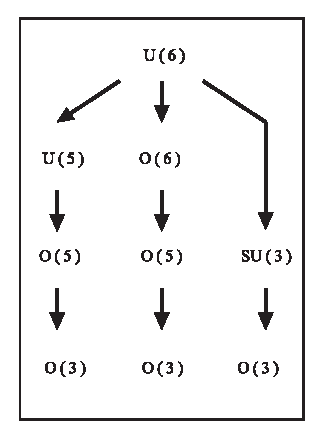
\includegraphics[scale=.65]{figure}
%
% If not, use
%\picplace{5cm}{2cm} % Give the correct figure height and width in cm
%
\caption{If the width of the figure is less than 7.8 cm use the \texttt{sidecapion} command to flush the caption on the left side of the page. If the figure is positioned at the top of the page, align the sidecaption with the top of the figure -- to achieve this you simply need to use the optional argument \texttt{[t]} with the \texttt{sidecaption} command}
\label{fig:1}       % Give a unique label
\end{figure}


\paragraph{Paragraph Heading} %
Instead of simply listing headings of different levels we recommend to let every heading be followed by at least a short passage of text. Furtheron please use the \LaTeX\ automatism for all your cross-references and citations as has already been described in Sect.~\ref{sec:2}.

Please note that the first line of text that follows a heading is not indented, whereas the first lines of all subsequent paragraphs are.

For typesetting numbered lists we recommend to use the \verb|enumerate| environment -- it will automatically render Springer's preferred layout.

\begin{enumerate}
\item{Livelihood and survival mobility are oftentimes coutcomes of uneven socioeconomic development.}
\begin{enumerate}
\item{Livelihood and survival mobility are oftentimes coutcomes of uneven socioeconomic development.}
\item{Livelihood and survival mobility are oftentimes coutcomes of uneven socioeconomic development.}
\end{enumerate}
\item{Livelihood and survival mobility are oftentimes coutcomes of uneven socioeconomic development.}
\end{enumerate}


\subparagraph{Subparagraph Heading} In order to avoid simply listing headings of different levels we recommend to let every heading be followed by at least a short passage of text. Use the \LaTeX\ automatism for all your cross-references and citations as has already been described in Sect.~\ref{sec:2}, see also Fig.~\ref{fig:2}.

Please note that the first line of text that follows a heading is not indented, whereas the first lines of all subsequent paragraphs are.

For unnumbered list we recommend to use the \verb|itemize| environment -- it will automatically render Springer's preferred layout.

\begin{itemize}
\item{Livelihood and survival mobility are oftentimes coutcomes of uneven socioeconomic development, cf. Table~\ref{tab:1}.}
\begin{itemize}
\item{Livelihood and survival mobility are oftentimes coutcomes of uneven socioeconomic development.}
\item{Livelihood and survival mobility are oftentimes coutcomes of uneven socioeconomic development.}
\end{itemize}
\item{Livelihood and survival mobility are oftentimes coutcomes of uneven socioeconomic development.}
\end{itemize}

\begin{figure}[t]
\sidecaption[t]
% Use the relevant command for your figure-insertion program
% to insert the figure file.
% For example, with the option graphics use
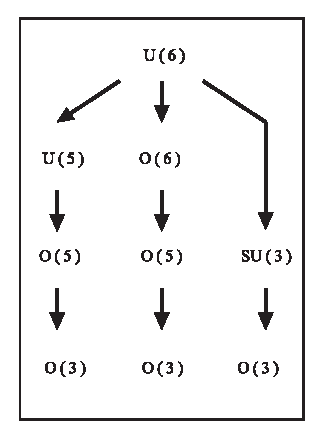
\includegraphics[scale=.65]{figure}
%
% If not, use
%\picplace{5cm}{2cm} % Give the correct figure height and width in cm
%
\caption{Please write your figure caption here}
\label{fig:2}       % Give a unique label
\end{figure}

\runinhead{Run-in Heading Boldface Version} Use the \LaTeX\ automatism for all your cross-references and citations as has already been described in Sect.~\ref{sec:2}.

\subruninhead{Run-in Heading Boldface and Italic Version} Use the \LaTeX\ automatism for all your cross-refer\-ences and citations as has already been described in Sect.~\ref{sec:2}\index{paragraph}.

\subsubruninhead{Run-in Heading Displayed Version} Use the \LaTeX\ automatism for all your cross-refer\-ences and citations as has already been described in Sect.~\ref{sec:2}\index{paragraph}.
% Use the \index{} command to code your index words
%
% For tables use
%
\begin{table}[!t]
\caption{Please write your table caption here}
\label{tab:1}       % Give a unique label
%
% For LaTeX tables use
%
\begin{tabular}{p{2cm}p{2.4cm}p{2cm}p{4.9cm}}
\hline\noalign{\smallskip}
Classes & Subclass & Length & Action Mechanism  \\
\noalign{\smallskip}\svhline\noalign{\smallskip}
Translation & mRNA$^a$  & 22 (19--25) & Translation repression, mRNA cleavage\\
Translation & mRNA cleavage & 21 & mRNA cleavage\\
Translation & mRNA  & 21--22 & mRNA cleavage\\
Translation & mRNA  & 24--26 & Histone and DNA Modification\\
\noalign{\smallskip}\hline\noalign{\smallskip}
\end{tabular}
$^a$ Table foot note (with superscript)
\end{table}
%
\section{Section Heading}
\label{sec:3}
% Always give a unique label
% and use \ref{<label>} for cross-references
% and \cite{<label>} for bibliographic references
% use \sectionmark{}
% to alter or adjust the section heading in the running head
Instead of simply listing headings of different levels we recommend to let every heading be followed by at least a short passage of text. Furtheron please use the \LaTeX\ automatism for all your cross-references and citations as has already been described in Sect.~\ref{sec:2}.

Please note that the first line of text that follows a heading is not indented, whereas the first lines of all subsequent paragraphs are.

If you want to list definitions or the like we recommend to use the Springer-enhanced \verb|description| environment -- it will automatically render Springer's preferred layout.

\begin{description}[Type 1]
\item[Type 1]{That addresses central themes pertainng to migration, health, and disease. In Sect.~\ref{sec:1}, Wilson discusses the role of human migration in infectious disease distributions and patterns.}
\item[Type 2]{That addresses central themes pertainng to migration, health, and disease. In Sect.~\ref{subsec:2}, Wilson discusses the role of human migration in infectious disease distributions and patterns.}
\end{description}

\subsection{Subsection Heading} %
In order to avoid simply listing headings of different levels we recommend to let every heading be followed by at least a short passage of text. Use the \LaTeX\ automatism for all your cross-references and citations citations as has already been described in Sect.~\ref{sec:2}.

Please note that the first line of text that follows a heading is not indented, whereas the first lines of all subsequent paragraphs are.

\begin{svgraybox}
If you want to emphasize complete paragraphs of texts we recommend to use the newly defined Springer class option \verb|graybox| and the newly defined environment \verb|svgraybox|. This will produce a 15 percent screened box 'behind' your text.

If you want to emphasize complete paragraphs of texts we recommend to use the newly defined Springer class option and environment \verb|svgraybox|. This will produce a 15 percent screened box 'behind' your text.
\end{svgraybox}


\subsubsection{Subsubsection Heading}
Instead of simply listing headings of different levels we recommend to let every heading be followed by at least a short passage of text. Furtheron please use the \LaTeX\ automatism for all your cross-references and citations as has already been described in Sect.~\ref{sec:2}.

Please note that the first line of text that follows a heading is not indented, whereas the first lines of all subsequent paragraphs are.

\begin{theorem}
Theorem text goes here.
\end{theorem}
%
% or
%
\begin{definition}
Definition text goes here.
\end{definition}

\begin{proof}
%\smartqed
Proof text goes here.
%\qed
\end{proof}

\paragraph{Paragraph Heading} %
Instead of simply listing headings of different levels we recommend to let every heading be followed by at least a short passage of text. Furtheron please use the \LaTeX\ automatism for all your cross-references and citations as has already been described in Sect.~\ref{sec:2}.

Note that the first line of text that follows a heading is not indented, whereas the first lines of all subsequent paragraphs are.
%
% For built-in environments use
%
\begin{theorem}
Theorem text goes here.
\end{theorem}
%
\begin{definition}
Definition text goes here.
\end{definition}
%
\begin{proof}
%\smartqed
Proof text goes here.
%\qed
\end{proof}
%
%
\begin{trailer}{Trailer Head}
If you want to emphasize complete paragraphs of texts in an \verb|Trailer Head| we recommend to
use  \begin{verbatim}\begin{trailer}{Trailer Head}
...
\end{trailer}\end{verbatim}
\end{trailer}
%
\begin{question}{Questions}
If you want to emphasize complete paragraphs of texts in an \verb|Questions| we recommend to
use  \begin{verbatim}\begin{question}{Questions}
...
\end{question}\end{verbatim}
\end{question}
%
%
\begin{important}{Important}
If you want to emphasize complete paragraphs of texts in an \verb|Important| we recommend to
use  \begin{verbatim}\begin{important}{Important}
...
\end{important}\end{verbatim}
\end{important}
%
\clearpage
\begin{warning}{Attention}
If you want to emphasize complete paragraphs of texts in an \verb|Attention| we recommend to
use  \begin{verbatim}\begin{warning}{Attention}
...
\end{warning}\end{verbatim}
\end{warning}

\begin{programcode}{Program Code}
If you want to emphasize complete paragraphs of texts in an \verb|Program Code| we recommend to
use

\verb|\begin{programcode}{Program Code}|

\verb|\begin{verbatim}...\end{verbatim}|

\verb|\end{programcode}|

\end{programcode}
%
\begin{tips}{Tips}
If you want to emphasize complete paragraphs of texts in an \verb|Tips| we recommend to
use  \begin{verbatim}\begin{tips}{Tips}
...
\end{tips}\end{verbatim}
\end{tips}
%
%
\begin{overview}{Overview}
If you want to emphasize complete paragraphs of texts in an \verb|Overview| we recommend to
use  \begin{verbatim}\begin{overview}{Overview}
...
\end{overview}\end{verbatim}
\end{overview}
\clearpage
\begin{backgroundinformation}{Background Information}
If you want to emphasize complete paragraphs of texts in an \verb|Background|
\verb|Information| we recommend to
use

\verb|\begin{backgroundinformation}{Background Information}|

\verb|...|

\verb|\end{backgroundinformation}|
\end{backgroundinformation}
\begin{legaltext}{Legal Text}
If you want to emphasize complete paragraphs of texts in an \verb|Legal Text| we recommend to
use  \begin{verbatim}\begin{legaltext}{Legal Text}
...
\end{legaltext}\end{verbatim}
\end{legaltext}
%
\begin{acknowledgement}
If you want to include acknowledgments of assistance and the like at the end of an individual chapter please use the \verb|acknowledgement| environment -- it will automatically render Springer's preferred layout.
\end{acknowledgement}
%
\section*{Appendix}
\addcontentsline{toc}{section}{Appendix}
%
When placed at the end of a chapter or contribution (as opposed to at the end of the book), the numbering of tables, figures, and equations in the appendix section continues on from that in the main text. Hence please \textit{do not} use the \verb|appendix| command when writing an appendix at the end of your chapter or contribution. If there is only one the appendix is designated ``Appendix'', or ``Appendix 1'', or ``Appendix 2'', etc. if there is more than one.

\begin{equation}
a \times b = c
\end{equation}
% Problems or Exercises should be sorted chapterwise
\section*{Problems}
\addcontentsline{toc}{section}{Problems}
%
% Use the following environment.
% Don't forget to label each problem;
% the label is needed for the solutions' environment
\begin{prob}
\label{prob1}
A given problem or Excercise is described here. The
problem is described here. The problem is described here.
\end{prob}

\begin{prob}
\label{prob2}
\textbf{Problem Heading}\\
(a) The first part of the problem is described here.\\
(b) The second part of the problem is described here.
\end{prob}

%%%%%%%%%%%%%%%%%%%%%%%% referenc.tex %%%%%%%%%%%%%%%%%%%%%%%%%%%%%%
% sample references
% %
% Use this file as a template for your own input.
%
%%%%%%%%%%%%%%%%%%%%%%%% Springer-Verlag %%%%%%%%%%%%%%%%%%%%%%%%%%
%
% BibTeX users please use
% \bibliographystyle{}
% \bibliography{}
%
\biblstarthook{In view of the parallel print and (chapter-wise) online publication of your book at \url{www.springerlink.com} it has been decided that -- as a genreral rule --  references should be sorted chapter-wise and placed at the end of the individual chapters. However, upon agreement with your contact at Springer you may list your references in a single seperate chapter at the end of your book. Deactivate the class option \texttt{sectrefs} and the \texttt{thebibliography} environment will be put out as a chapter of its own.\\\indent
References may be \textit{cited} in the text either by number (preferred) or by author/year.\footnote{Make sure that all references from the list are cited in the text. Those not cited should be moved to a separate \textit{Further Reading} section or chapter.} If the citatiion in the text is numbered, the reference list should be arranged in ascending order. If the citation in the text is author/year, the reference list should be \textit{sorted} alphabetically and if there are several works by the same author, the following order should be used:
\begin{enumerate}
\item all works by the author alone, ordered chronologically by year of publication
\item all works by the author with a coauthor, ordered alphabetically by coauthor
\item all works by the author with several coauthors, ordered chronologically by year of publication.
\end{enumerate}
The \textit{styling} of references\footnote{Always use the standard abbreviation of a journal's name according to the ISSN \textit{List of Title Word Abbreviations}, see \url{http://www.issn.org/en/node/344}} depends on the subject of your book:
\begin{itemize}
\item The \textit{two} recommended styles for references in books on \textit{mathematical, physical, statistical and computer sciences} are depicted in ~\cite{science-contrib, science-online, science-mono, science-journal, science-DOI} and ~\cite{phys-online, phys-mono, phys-journal, phys-DOI, phys-contrib}.
\item Examples of the most commonly used reference style in books on \textit{Psychology, Social Sciences} are~\cite{psysoc-mono, psysoc-online,psysoc-journal, psysoc-contrib, psysoc-DOI}.
\item Examples for references in books on \textit{Humanities, Linguistics, Philosophy} are~\cite{humlinphil-journal, humlinphil-contrib, humlinphil-mono, humlinphil-online, humlinphil-DOI}.
\item Examples of the basic Springer style used in publications on a wide range of subjects such as \textit{Computer Science, Economics, Engineering, Geosciences, Life Sciences, Medicine, Biomedicine} are ~\cite{basic-contrib, basic-online, basic-journal, basic-DOI, basic-mono}. 
\end{itemize}
}

\begin{thebibliography}{99.}%
% and use \bibitem to create references.
%
% Use the following syntax and markup for your references if 
% the subject of your book is from the field 
% "Mathematics, Physics, Statistics, Computer Science"
%
% Contribution 
\bibitem{science-contrib} Broy, M.: Software engineering --- from auxiliary to key technologies. In: Broy, M., Dener, E. (eds.) Software Pioneers, pp. 10-13. Springer, Heidelberg (2002)
%
% Online Document
\bibitem{science-online} Dod, J.: Effective substances. In: The Dictionary of Substances and Their Effects. Royal Society of Chemistry (1999) Available via DIALOG. \\
\url{http://www.rsc.org/dose/title of subordinate document. Cited 15 Jan 1999}
%
% Monograph
\bibitem{science-mono} Geddes, K.O., Czapor, S.R., Labahn, G.: Algorithms for Computer Algebra. Kluwer, Boston (1992) 
%
% Journal article
\bibitem{science-journal} Hamburger, C.: Quasimonotonicity, regularity and duality for nonlinear systems of partial differential equations. Ann. Mat. Pura. Appl. \textbf{169}, 321--354 (1995)
%
% Journal article by DOI
\bibitem{science-DOI} Slifka, M.K., Whitton, J.L.: Clinical implications of dysregulated cytokine production. J. Mol. Med. (2000) doi: 10.1007/s001090000086 
%
\bigskip

% Use the following (APS) syntax and markup for your references if 
% the subject of your book is from the field 
% "Mathematics, Physics, Statistics, Computer Science"
%
% Online Document
\bibitem{phys-online} J. Dod, in \textit{The Dictionary of Substances and Their Effects}, Royal Society of Chemistry. (Available via DIALOG, 1999), 
\url{http://www.rsc.org/dose/title of subordinate document. Cited 15 Jan 1999}
%
% Monograph
\bibitem{phys-mono} H. Ibach, H. L\"uth, \textit{Solid-State Physics}, 2nd edn. (Springer, New York, 1996), pp. 45-56 
%
% Journal article
\bibitem{phys-journal} S. Preuss, A. Demchuk Jr., M. Stuke, Appl. Phys. A \textbf{61}
%
% Journal article by DOI
\bibitem{phys-DOI} M.K. Slifka, J.L. Whitton, J. Mol. Med., doi: 10.1007/s001090000086
%
% Contribution 
\bibitem{phys-contrib} S.E. Smith, in \textit{Neuromuscular Junction}, ed. by E. Zaimis. Handbook of Experimental Pharmacology, vol 42 (Springer, Heidelberg, 1976), p. 593
%
\bigskip
%
% Use the following syntax and markup for your references if 
% the subject of your book is from the field 
% "Psychology, Social Sciences"
%
%
% Monograph
\bibitem{psysoc-mono} Calfee, R.~C., \& Valencia, R.~R. (1991). \textit{APA guide to preparing manuscripts for journal publication.} Washington, DC: American Psychological Association.
%
% Online Document
\bibitem{psysoc-online} Dod, J. (1999). Effective substances. In: The dictionary of substances and their effects. Royal Society of Chemistry. Available via DIALOG. \\
\url{http://www.rsc.org/dose/Effective substances.} Cited 15 Jan 1999.
%
% Journal article
\bibitem{psysoc-journal} Harris, M., Karper, E., Stacks, G., Hoffman, D., DeNiro, R., Cruz, P., et al. (2001). Writing labs and the Hollywood connection. \textit{J Film} Writing, 44(3), 213--245.
%
% Contribution 
\bibitem{psysoc-contrib} O'Neil, J.~M., \& Egan, J. (1992). Men's and women's gender role journeys: Metaphor for healing, transition, and transformation. In B.~R. Wainrig (Ed.), \textit{Gender issues across the life cycle} (pp. 107--123). New York: Springer.
%
% Journal article by DOI
\bibitem{psysoc-DOI}Kreger, M., Brindis, C.D., Manuel, D.M., Sassoubre, L. (2007). Lessons learned in systems change initiatives: benchmarks and indicators. \textit{American Journal of Community Psychology}, doi: 10.1007/s10464-007-9108-14.
%
%
% Use the following syntax and markup for your references if 
% the subject of your book is from the field 
% "Humanities, Linguistics, Philosophy"
%
\bigskip
%
% Journal article
\bibitem{humlinphil-journal} Alber John, Daniel C. O'Connell, and Sabine Kowal. 2002. Personal perspective in TV interviews. \textit{Pragmatics} 12:257--271
%
% Contribution 
\bibitem{humlinphil-contrib} Cameron, Deborah. 1997. Theoretical debates in feminist linguistics: Questions of sex and gender. In \textit{Gender and discourse}, ed. Ruth Wodak, 99--119. London: Sage Publications.
%
% Monograph
\bibitem{humlinphil-mono} Cameron, Deborah. 1985. \textit{Feminism and linguistic theory.} New York: St. Martin's Press.
%
% Online Document
\bibitem{humlinphil-online} Dod, Jake. 1999. Effective substances. In: The dictionary of substances and their effects. Royal Society of Chemistry. Available via DIALOG. \\
http://www.rsc.org/dose/title of subordinate document. Cited 15 Jan 1999
%
% Journal article by DOI
\bibitem{humlinphil-DOI} Suleiman, Camelia, Daniel C. O'Connell, and Sabine Kowal. 2002. `If you and I, if we, in this later day, lose that sacred fire...': Perspective in political interviews. \textit{Journal of Psycholinguistic Research}. doi: 10.1023/A:1015592129296.
%
%
%
\bigskip
%
%
% Use the following syntax and markup for your references if 
% the subject of your book is from the field 
% "Computer Science, Economics, Engineering, Geosciences, Life Sciences"
%
%
% Contribution 
\bibitem{basic-contrib} Brown B, Aaron M (2001) The politics of nature. In: Smith J (ed) The rise of modern genomics, 3rd edn. Wiley, New York 
%
% Online Document
\bibitem{basic-online} Dod J (1999) Effective Substances. In: The dictionary of substances and their effects. Royal Society of Chemistry. Available via DIALOG. \\
\url{http://www.rsc.org/dose/title of subordinate document. Cited 15 Jan 1999}
%
% Journal article by DOI
\bibitem{basic-DOI} Slifka MK, Whitton JL (2000) Clinical implications of dysregulated cytokine production. J Mol Med, doi: 10.1007/s001090000086
%
% Journal article
\bibitem{basic-journal} Smith J, Jones M Jr, Houghton L et al (1999) Future of health insurance. N Engl J Med 965:325--329
%
% Monograph
\bibitem{basic-mono} South J, Blass B (2001) The future of modern genomics. Blackwell, London 
%
\end{thebibliography}


\motto{}
\chapter{Pervasive Concepts}
\label{intro03} % Always give a unique label
% use \chaptermark{}
% to alter or adjust the chapter heading in the running head

\abstract{
}

\section{Characteristics}
\label{sec:03:1}

Characteristics are containers that record a set of attribute values
(ex: number\_of\_drivers = 2, make\_of\_car = Honda, resale\_value=10000)
which a policy contract is based on, and additionally a time interval over which
those attribute values are valid. Abstractly, it's a combination of a map and a time
interval. 

Below we just consider the time interval part of a characteristics and detail
how those intervals split as the standard modification operations are applied
to intervals
\import{ch03/}{CharacteristicsSplitCtx0-sa.tex}
\import{ch03/}{CharacteristicsSplitMch0-sa.tex}

\section{Liquid Calculations}
\label{sec:03:2}

\import{ch03/}{CancellationCalculations-sa.tex}

\section{Intervals}
As you work with framework objects, you will soon come to see that most objects cover
an interval from $start\_timestamp$ to $end\_timestamp$. These times delineate an extent of
a coverage interval or in the case of a modification the times delineate the time range for
which a coverage change was requested.

There is also a second type of framework object which is very common and interval like. These
are temporal objects and are identifiable by the fields $issued\_timestamp$ and $replaced\_timestamp$.
More commonly you may have seen these fields in other frameworks by the names $valid\_from$ and
$valid\_to$. This simple structure is used to record an audit history and allow easy acquisition of the current set
of valid objects with a filter of the form
\begin{equation*}
issuedTimestamp \neq null \land replacedTimestamp = null
\end{equation*}

Here are some standard interval functions that are available for use in the framework.
\import{ch03/}{IntervalOps-sa.tex}

\section{Holdbacks}
\label{sec:03:3}

\subsection{Concept}

\begin{figure}[ht]
  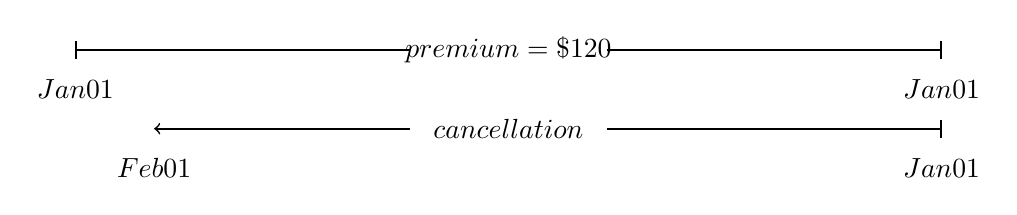
\begin{tikzpicture}
    \draw[|-,semithick] (0,-0.5) -- (4.25,-0.5);
    \draw (5.5, -0.5) node {$premium = \$120$};
    \draw[-|,semithick] (6.75,-0.5) -- (11,-0.5);
    \draw (0,-1) node {$Jan 01$};
    \draw (11,-1) node {$Jan 01$};
    
    \draw[<-,semithick] (1,-1.5) -- (4.25,-1.5);
    \draw (5.5, -1.5) node {$cancellation$};
    \draw[-|,semithick] (6.75,-1.5) -- (11,-1.5);
    \draw (1,-2) node {$Feb 01$};
    \draw (11,-2) node {$Jan 01$};
    
  \end{tikzpicture}   
  \caption{
    A policy and a cancellation
  }
  \label{fig:3:1}
\end{figure}

To explain holdbacks consider a policy running from Jan 1st of one year to Jan 1st of the next year, with a
premium of 120 dollars. If
a customer decided to cancel this policy starting at Feb 1st, then there are two adjustments that would
be made to this policy. First the premium would be prorated to account for the single month of coverage.
Assuming monthly proration 10 dollars would be charged for the month of coverage. Next there may be penalty
charges due to the customer canceling the policy early. We call these penalty charges holdbacks, and a typical
charge scenario, for our example, might be:
\begin{eqnarray*}
totalCharges_{Jan01->Feb01} & = & prorated(premium) + holdback \\
                          & = & (\frac{1}{12}) premium + 0.1(\frac{11}{12})(premium)
\end{eqnarray*}
where, here, the customer is charged a ten percent penalty fee on the part of the policy that was cancelled.


\subsection{Specification}

Below is Socotra mathematical specification for holdbacks
\import{ch03/}{ProrationCtx2-sa.tex}
\import{ch03/}{ProrationMch2-sa.tex}


\motto{Seek not to have things happen as you choose them, but rather choose them to happen as they do.}
\chapter{Cancellation and Renewal}
\label{intro} % Always give a unique label
% use \chaptermark{}
% to alter or adjust the chapter heading in the running head

\abstract{During the course of a policy's lifetime it may be necessary to cancel a policy because invoices have not been paid or for other
  business reasons. These same policies may then need to be restored to their state before the cancellation. The cancellation and
  renewal functionality in the Socotra system handles these policy changes. \newline\indent
  The functionality operates through two distinct mechanism. The first is though API which customers use to trigger cancellations or reinstatements.
  There is also a group of automated jobs which can cancel a policy or reinstate it when a policies state satisfies certain lifecycle conditions.
}

\section{Overview}
\label{sec:02:1}
In our discussion of policies so far we dealt with the modifications
\begin{equation*}
  \{Creation, Endorsement, Renewal\}.
\end{equation*}
To this set we now
add the modifications
\begin{equation*}
  \{Cancellation, Reinstatement\}.
\end{equation*}
These new modifications are similiar to modifications we already
know, with slight differences. Reinstatements are different in that they have two unique fields, described below, and Cancellations
are different in that their state lifecycle only has the two events onCreate and onIssue. Below is the general context in which
we can start to model the cancellation and renewal module.

\import{ch02/}{CancellationCtx1-sa.tex}

With the new modifications modeled we can now lay out actions on our policy in the usual state centric way. Cancellations with have
onCreate and onIssue events that they respond to. And Reinstatements respond to onCreate, onAccept and onIssue events. 

\import{ch02/}{CancellationMch1-sa.tex}

\section{Liquid Calculations}
\label{sec:02:2}

\import{ch02/}{CancellationCalculations-sa.tex}

\motto{}
\chapter{Scheduled Jobs}
\label{intro} % Always give a unique label

\abstract{}

\section{Grace and Lapse}
\label{sec:jobs:1}
In addition to cancellations that can happen through the API, it's also possible to policies to be canceled automatically by
the system. This automated cancellation happens when a policy has outstanding invoices which have not been paid. The system
scheduled grace job flags outstanding invoices and the scheduled lapse job after some time will eventually cancel the policies
associated with those flagged invoices. Below is a simplified model of the process, which details the essential points of
understanding for the jobs.
\import{chJobs/}{AutoGraceLapseInvoiceCtx0-sa.tex}
\import{chJobs/}{AutoGraceLapseInvoiceMch0-sa.tex}

\section{Document Consolidation}
\label{sec:jobs:2}
\import{chJobs/}{DocConsolidateCtx0-sa.tex}
\import{chJobs/}{DocConsolidateMch0-sa.tex}



\begin{partbacktext}
\part{Systems and Applications}
\noindent We review Socotras systems. We discuss how they are structured in the large, and what structuring might be an improvement.
Some documentation on specific system applications is presented.

\end{partbacktext}

\motto{To learn to make art you spend time working with the materials. That is it. When the urge arises to judge the quality of 
  your work, it will be tempting to say this is good or this is bad. Take that energy that you might put into assessing 
  the aesthetic and put it back into the materials instead. Persist and grow. Avoid aesthetic judgements, and instead
  produce work.}
\chapter{The Systems}
\label{intro:04} % Always give a unique label
% use \chaptermark{}
% to alter or adjust the chapter heading in the running head

\abstract{
  Socotra has a very simple system setup. There are two user interfaces and a few backend
  systems, the most important of which is the API. The biggest problem with understanding
  the system setup is that the names of the components don't always imply what the component
  does. The description, below, will match up components with a function and where possible
  indicate some reasonable naming.
}

\section{Structure of the Overall System}
\label{sec:04:1}

\import{ch04/}{SystemOrganization.tex}

Figure 3.1 shows the overall system. The Config Editor is a policy designer. From within Config
Editor product experts can define insurance products as a combination of json configuration
files, tables for value lookup, and script files for dynamic policy calculations. Once a product
is defined and deployed, then the Policy Manager is used by company representative to create
policy holders and to issue and modify policies based on a product.

Load Assets is part of the backend. It accepts zipped product, configuration files from Config Editor and
it orchestrates the deployment of those product, configuration files using internal APIs that the
Socotra API exposes. The Socotra API is then a very standard API application. It stores data in
a few external databases. And it relies on a javascript executor called Socol to do dynamic calculations,
for instance fees or taxes.

\section{Structure of Socotra API}
\label{sec:04:2}
\import{ch04/}{ApiOrganization.tex}

The Socotra API application is a simple layered application built on the Spring Framework. The
layering is somewhat unconventional; however, which makes the structure not immediately evident.
Figure 3.2 shows the current API structure with a generic application structure for comparison. The
best way to think of the Socotra API is as having a very thin controller layer at the front and a
very thin layer at the back of request and response objects, that are used everywhere. Then
there is a very thick middle layer which contains everything else. The application could certainly use
more circumspect layering to organize code and developer thinking. It's likely that the application
will evolve over time to look more and more like the generic application structure on the right.
In fact, its unlikely that anything more nuanced could be needed.






\motto{\dots and now each one went the way upon which he had decided, and they set
out into the forest at one point or another, there where they saw it to be thickest.}
\chapter{Developing the Applications}
\label{intro05} % Always give a unique label
% use \chaptermark{}
% to alter or adjust the chapter heading in the running head

\abstract{
  Doing work
}

\section{Config Manager}
\import{ch05/}{ReadMeConfigManager-sa.tex}

\section{Policy Editor}
\import{ch05/}{ReadMePolicyEditor-sa.tex}

\section{Load Assets}
\import{ch05/}{ReadMeLoadAssets-sa.tex}
\import{ch05/}{LoadAssetsApi-sa.tex}
\import{ch05/}{LoadAssetsTrafficAnalysis-sa.tex}

\section{Python Client}
\import{ch05/}{ReadMePythonClient-sa.tex}
\import{ch05/}{PythonClientUsingFromPythonCode-sa.tex}
\import{ch05/}{PythonClientUsingTheUtilityPrograms-sa.tex}

\section{Stack Api Service}
\import{ch05/}{ReadMeStackApiService-sa.tex}



\appendix
\motto{Sin bravely.}
\chapter{Extra stuff that I hope might help}
\label{introA} % Always give a unique label

\section{Engineering Practices}
\label{sec:A1}
Over the years of doing engineering, we all come away with different learnings and a view of the task shaped by our experiences.
Below are some thoughts I have about engineering which have grow out of my experiences and condensed into topics. Perhaps some
of the topics will resonate with you and become part of your experience. The summary is below and details follow:
\begin{enumerate}
\item Define the problem. The problem you have isn't the problem you think you have.
\item Build in minimal commits.
\item If you don't understand all observations, then your understanding is wrong.
\item If code is not being used, then it doesn't work.
\item System problems can not be solved with single solutions, or by efforts at a single time.
\item Change one thing at a time.
\item There is no right way. There are only trade offs.
\item Build your personal rule set.
\item If you don't know what to do, then do something anyways.
\item Theory and practice.
\end{enumerate}

\subsection{Define the Problem.}
\label{sec:A2}
It should be axiomatic that if one cant define a problem, one cant solve it. It should be equally clear that if one defines a
problem incorrectly, then regardless of the quality of the solution one provides, the solution provides no value in the context of
the actual need.
As obvious as the above statements are, you should not deceive yourself into thinking that the ability to define
problems is natural, and even less that a problem, when it reaches your desk, has been correctly defined as stated. One should, in fact,
assume just the opposite.
In the course of your career, unless you are finding that 90 percent of the time your problems have to be reexamined and refined,
then it's probable you are not thinking carefully enough before you work.

Let's think through a current, discussion topic at Socotra, feature flags, to illustrate defining a problem. I don't happen to know what the
resolution to the feature flag ``problem'' will be and perhaps that is good. You, the future reader with hindsight and proof of time, will
all the better be able to evaluate the usefulness of the thoughts on problem definition that follow.

Lets start with a real life, feature flag problem statement that we can quickly disregard.
\begin{description}
\item[Problem] The current feature flag
mechanism (with flags in database tables) is inelegant.
\end{description}
Perhaps no one has made exactly this feature flag problem statement. But statements like this have been thrown about and, of course as
developers, we love to disparage the technologically ugly with variants of this statement. Now, I am not sure what the official engineering
definition of inelegant is. If it had an engineering definition, I am not convinced that such a label would be sufficient to establish the
existence of a problem. Inelegant is an aesthetic, emotional judgment, and while there is room for aesthetics in engineering, we should be
on our guard. Feature flags presumably would fulfill a functional need and not an aesthetic, emotional need. Let's try again.

\begin{description}
\item[Problem] Lets investigate the Launch Darkly feature flag functionality to see how it could be used in our current systems.
\end{description}
This statement is an example of a solution with an assumed problem. The problem could exist, but for the author of the statement above
it seems his solution is so obvious and perfect that he
has skipped the trivial formality mentioning it. As an engineer you should sensitize yourself to solutions that eclipse their problems.
``We should build new functionality as micro services'' or
``We should use Amazon Lambda for X, because Lambda is scalable and the future of software development'' are other examples. I am sure Launch Darkly is wonderful,
as well as micro services and Amazon Lambda, and yet their wonderfulness does not mandate their use. As an engineer, when technical discussion 
leads directly to technical implementation X or a technology Y, that is a tell that perhaps someone had a vague feeling about a
problem and the source of that feeling was easiest for them to express as the absence of a technology, for instance ``MongoDB''. (And as the joke goes, now
you have two problems).

Since we achieved insufficient clarity with the above problem definitions let's metaphorically go back to the beginning and talk about feature
flags. Feature flags are a soft deployment mechanism, which activate software functionality. Feature flags complement and add additional
flexibility to physical deployment mechanisms. In any existing implementation, the flag consists of a name and associated data (Boolean,
Enumerated...) stored in persistence somewhere. Is that elegant? We can list some of the common problems that feature flags solve. I took
the following problems from the web site of a commercial service that sells a feature flag management product. I believe the list is complete.

\begin{description}
  \item[Problem 1] A mechanism is needed to rollout software incrementally (for example: 10\% of users, 20\% of users,\dots) while monitoring
  metrics for errors or performance problems.
  \item[Problem 2] A short lived mechanism is needed to enable subsets of users to see different site functionality, perhaps for the purpose of
  running experiments.
  \item[Problem 3] A mechanism is needed to reconfigure code and it is not practical or desirable to do this via physical deployments.
\end{description}
Briefly reflect on how the above problems apply to Socotra. And with that reflection done, let's define Socotra's
problems.

Since feature flags are just a deployment mechanism, let's not immediately bring feature flags into our problem definition exercise, as we might
fool ourselves into
talking about a solution. Instead lets talk about what needs Socotra has around deployment functionality. Here is one deployment problem I
have witnessed at Socotra
\begin{description}
  \item[Problem] A mechanism is needed to rollout software incrementally (for example: organization \#1, a few days later organization \#2, \dots) while monitoring
  metrics for errors or performance problems.
\end{description}
For the instance where the above problem came up, Devops could have made incremental physical deployments but since the rollout had
more than one moving part it was conceptually simpler to put all the pieces in place and then flip a flag to bring everything live.
A database table, \_env\_feaure, supplied the global, boolean feature flag to bring the new functionality live and that mechanism was
simple and sufficient. There were no problems. That said, I can envision a more complex Socotra system where functionality might be
deployed in independent components in pieces; where one flag to bring all component functionality live at once, would enable conceptually simple deployment;
and where a flag in a database table would not be available to all the components. That would pose a deployment problem. We would probably
want to be aware of that future problem and address it at the proper time according to our engineering judgment.

In contrast, here is another common deployment problem I am aware of at Socotra
\begin{description}
  \item[Problem] Wonderful new functionality X has been developed and insurance companies are dying to start using it. Unfortunately insurance companies
  cant readily use the new functionality because the new functionality requires that new fields or a new file be added to the product configuration. Even
  though insurance companies have deployed new product configurations, all their existing policies are tied to the previous product revision. They have to wait for each
  policy to be renewed, maybe a year, until they and their policyholders can all enjoy wonderful new functionality. It's very inconvenient for insurance
  companies, their systems, and their policyholders to receive functionality in this manner.
\end{description}
This is a problem that is immanent once product versioning goes live. Today this problem  is more salient than any other deployment problem Socotra
has and as engineers we should have immanent problems clear in our minds. Again, I am going to leave the solution to this problem to the reader,
but we might observe that practical engineering, perhaps not elegance and certainly not Launch Darkly, will be involved in the solution. We might also observe
that, exactly like feature flags, the deployment of configuration zip files is a type of soft deployment, which complements and adds additional
flexibility to physical deployments mechanisms.

I will leave the exercise there. There is more to say. There are tenant level flags and request level flags. But that belabors the point to make
which is that
one should get into the habit of turning over a problem statement in ones mind, formulating it from various angles and reducing it to
essentials. In your career as an Engineer it is important that you be successful, and one of the keys skills that will guide you towards doing what should
be done, and assist co-workers with business skill sets is the ability to clearly and correctly define what the problem is.


\subsubsection{Build in minimal commits.}
I am often surprised, when I model a system with a computer checked tool, by how difficult it is to get the model correct. Usually the model
is highly abstracted and simplified, a toy compared to the real thing. And yet the tools find corner cases that I would never have discovered with
human reasoning skills. The reason for the surprise is that as engineers, and more so for non engineers, we have only a passing feeling for the
ability of state to multiply. Consider the simple, cancellation model in Chapter 2. How many states are there if the model steps through 8 time intervals?
There are almost a million and the model checker takes half and hour to check them all of them.

You are not impressed perhaps. We already know software is complex. This afternoon, I sat through an engineering discussion where an ongoing systems problem
was brought up:
``Its hard for me to predict the effects of my changes \dots'', because system bad. A few months ago I sat through a related engineering discussion about how
difficult it is to estimate delivery dates for new and ongoing projects, because system bad. What we need is? \- to have better encapsulation, to move the system
towards a micro-service architecture, to design with better architecture and patterns \dots or add your own favorite delusion. I am going to suggest an alternate theory for system
bad based on my frustrations building simple, abstract mathematical models. I will suggest that you are a very limited human being in the face of what you have created, and you have
to learn to work in a way that is appropriate to that reality.

Now, I know you are an experienced engineer, and you have read all the books, and you have come through the toughest, largest projects there are. You already
know what you are doing. And still there may be just one more practice that no one has ever told you and in fact its just the opposite of what the people who
talk cleaner code, and micro-service architecture, and design patterns propagandize. The practice is: make minimal commits. If you have a bug, or if you have
a feature to implement, or if you have a project to finish, find the smallest problem related to your bug, feature or project and define it precisely.
Write code to solve just that problem, precisely. Commit. Repeat until you are done. Anything can be accomplished as a series of minimal commits.

I know you will be tempted to disregard this practice. The minimum. That sounds so negligent. Why you may even desire to refactor. After all that was promoted in those
books about clean code, micro-services and patterns and stuff; the guys that wrote those books really know what they are doing, right? Well, I am not telling you to do the minimum. I am not telling
you to not make systems better. What I am saying is you are limited. You didn't 100\% understand the ramifications of that ambitious bug fix you made today and,
by the way, you didn't sleep well last night. That ambitious architecture idea you've been thinking on; two years from now you are going to look back and think
it was foolish, because you have grown. I am saying if you are limited, a precise, rigorous practice will help you be successful, and I am afraid other engineers
you meet in your career are not going to tell you. Minimal commits. Precisely define the minimal problem, write just that code, and commit. A lot of tasks
become better executed, a lot of systems improve, and you will be more successful if you can just repeat that process.

\subsection{If you don't understand all observations, then your understanding is wrong.}
One of the traits of a good theory is that when you apply it to a phenomena you are investigating, then it explains all of the observations you have made, not 90\%
of your observations, not 95\% of you observations, all of your observations. One of the traits of a bad theory is that it explains enough to
satisfy you. The classic example of a bad theory is Ptolemy's geocentric model of the universe. It explained almost all heavenly observations and served as the basis
for precise astronomical calculations. It was satisfactory enough. One just ignored the last few percent of observations that didn't make any sense. Now, stop for a
second and imagine yourself believing the geocentric model of the universe. Are you mostly correct in your understanding of the universe or do you know
essentially nothing about the universe?

If you have lived long enough, you can dip into your memories of past, very reasonable, theories which did not quite pan out. When I was growing up, I had an Aunt
who had a subscription to National Geographic, a very reputable magazine at the time. Sometime in the 70's I remember National Geographic running a whole magazine
detailing the case for an impending famine in the US. Back in the 70's it was also assured knowledge that the world would run out of oil sometime in the early 1990s.
In retrospect,
National Geographic knew essentially nothing about famine. Assured knowledge knew essentially nothing about the availability of energy resources on the planet. And yet
the theories accounted for most to the facts. How can that be? What you have to realize is that mismatches between observations and theories have to
drop your confidence in your theory a lot. If you have 10 observations and your theory explains 9 of those observations. As much as you'd like to,
you should not have 90\% confidence in your theory. You should have more like 50\% confidence. If you can explain 8 observations, you should have more like 25\%
confidence in your theory. Put another way you need more explanatory power than you think before you know more than nothing.

Now lets talk about theories in relation to computer systems at Socotra. I am going to recount a story from a few months ago. I was in Socotra's daily scrum and an engineer
explained that he was working on a bug. He explained that he couldn't quite reproduce the error or detail how the error was coming about. But he was pretty confident
that the ultimate cause had to be X and he had committed a solution Y. That is bad practice, and it is all too common among software engineers. Software engineering culture
accepts and allows people to make the jump from ``my theory explains an observation'' to ``my theory is correct''. This jump is not acceptable or allowed in any other
engineering discipline. Unless you can reproduce, unless you can explain, unless you can account for all the observations, then you know nothing. You need to
dig deeper, and you have no business committing solution Y, except to gain missing data.

Above we talked about when a bug is properly understood and hopefully corrected. On a related note, and getting back to the title of this post, imagine you are writing
code, building a system. Further, imagine that in one of the system executions you notice something curious. Possibly an error, but you cant reproduce it. And you are very busy;
it's probably something one off. I am going to suggest that your understanding of your code is like a theory and you have an observation that contradicts the
theory. With that one contradiction, you now need more explanatory power than you think to assume something one off happened. In fact, despite your
best feelings of assurance, you have to assume, with assurance, that the code is wrong. And do work to generate an explanation.

What I have written above might seem a bit strong. If it seems a bit strong then for your next few bugs fixes, start by listing all you theories. Maybe
you will start off with 10 possible theories and you might well add new theories as you work through the bug. Note that you will generally have to toss
away a lot of plausible theories before you finally find a root cause of your bug. Note also that the solution that you finally end with, will not generally be
in the initial set of theories you started with. What I have written above might, on the other hand, seem obvious. If that is that case, then the next time
you read the news just take note of topics of current concern and the related theories, sufficient for you to feel assured in your opinions. (Covid and Global
Warming are on the front page of CNN as I write this.) Then come back to this paragraph in 15 years.

\subsection{If code is not being used, then it doesn't work.}
When building systems its common to have unused code: sub-systems that are finished, waiting to go live or code that is not
executed on a regular basis. Any code that one expects to work must prove it works on a regular basis. If the code does not prove it works, your best assumption
is that it does not.

\subsection{System problems can not be solved with single solutions, or by efforts at a single time.}
In a recent engineering meeting development quality was evaluated in terms of the number of customer bug reports per month.
One tentative suggestion from the graphs was that there was a large number of latent bugs in existing code waiting to be exposed by
new customers doing new things. This prompted the question of how can we remove bugs from the existing code and the response was
``we have to write more tests''. How likely is that to be a solution for uncovering latent bugs in code?

We can answer questions like this by making a quick engineering estimates. How many state items are there in the configuration plus
database fields that can influence processing? Lets say the state items are bounded on the low side by $10^2$. Lets further assume
that all states are binary and
that processing is never influenced by the confluence of more than three data items. The system then has a lower bound of $10^6$ state combinations.
If not properly handling some of those $10^6$ states would lead to a bug, then we can say that to sufficiently
remove just data bugs, a lower limit on the number of tests necessary would be $10^6$. Further we would still have many other classes of bugs
to investigate with perhaps equally large state spaces. No team will ever write those tens of millions of tests, and if they could then they would
spend months of time just trying to run their test suite, once. The answer ``we have to write more tests'' does not work in theory. Slightly differently,
theory tells you a given solution is wrong.

I am going to give you another answer to the question of how to remove bugs in existing code. But the answer is general to all improvements
that one seeks to implement in complex systems. You have to accumulate a set of effective attack methods to use towards your goal and
you have to apply those methods systematically over an extended period of time. The extended period of time varies by the problem domain
but for software systems a typical value of the extended period of time is on the order of one year.

When I started my first job as a software engineer, I worked at a financial institution in Boston with a faulty reporting system. It was a big
problem because customers expected timely (right now) financial reports and there were ten to fifty failures that had to be resolved every morning. Every
morning I would try to identify every problem and manually produce the reports by any means necessary. Then I would go downstairs to my
desk and fix as many problems as were identified. I would also search all the other reports for any specific classes of problems that could be
extrapolated from the days failures and I would fix those too. For some issues I would ask ``what would I have to do to prevent an issue like
this from ever happening again?'' and then I would do that. For issues that I couldn't find a root cause for, I had a lab notebook where I
would record every issue and every observation that I had made about the issue. Everything was tracked. Where I needed more information,
I would add logging and monitoring. After a year of persistent attack from many angles, one day I came into work and there were no report
failures. Over the years, with many failing systems I have personally seen variations of the above story replay many times. There are no easy one
shot solutions. One applies many simple strategies, consistently over time, and in about a year one will end up where one wants to be.

\subsection{Change one thing at a time.}
Most systems, even simple systems are complex enough to exceed the reasoning ability of the best engineers, and we can see the manifestation of this truth regularly at
Socotra. We have a moderately complex system and yet its not unknown to see one or more engineers struggle to fix system problems and
be uncertain about the ultimate fix. Will the fix be correct in all circumstances? It's also not unknown for specifications of new functionality
to be incomplete or in need of revision after discussion of system details. Demonstrably, no one can reason about our system with confidence, and
I would suspect that the most confident are in line to fall the hardest.

One golden rule for navigating system complexity (along with minimal commits) is to always change one thing at a time. If someone changes module
X and you would like to add functionality in module X for your feature, Y. Wait for X to go live in production and then add your feature Y. If
problems occur in Module X or a related module before your changes land, then someone else is closer to isolating what changes have created problems.
It's always much harder to analyze a problem when multiple changes have happened at the same time especially if the changes interact in
unintuitive ways. One change at a time is also why many organizations deploy code continuously. If each commit is well targeted, which it should
be, then only one piece of functionality has changed. If after a deployment, monitors show abnormalities, then code can be rolled back and it will
be very apparent what single change caused what problem. Surprisingly what seems to be very dangerous, deploying as soon as commits land, turns
out to be safer because only one thing is changing at a time.

\subsection{There is no right way. There are only trade offs.}
Try never to say ``this is the right way to do it''. That statement may be emotionally satisfying but it is not engineering. Engineering
is about trade offs. Just like raising children or like deciding what to do on the weekend or like deciding what business opportunities to pursue.
One defines the problem (see above) or, mathematically, one defines a set of inequalities which bound the solution space. One then navigates among needs,
values, precise discussion with stakeholders, and hopefully good judgment to pick a point in that solution space. Being an engineer means you
can come up with many possible solutions to any problem and you can explain the trade off for each one.

\subsection{Build you personal rule set.}
When you work on complex systems try to find rules that can guide you in your interaction with that system. All interactions with complex systems
that have survived through the ages do precisely this. In human society the rules that guide interaction are called culture. In governance the
rules that guide interactions will be conventions like parliamentary procedures, rule of law, and freedom of speech. In an economic
system one rule might be voluntary exchange. The rules exist not because they are perfect but because they have been found to work well most
of the time. And because human judgment is not sound enough to distinguish the exceptional cases. Similarly when you code or modify systems think about the
rules that should guide you in your changes. If you create a bug perhaps you should have a rule for each bug you fix you must write a unit
test. That's a common rule that a lot of engineers have. If you have to make a change to a system you might decide that as a rule you will identify
the minimal fix, as discussed. And code just that. You might decide that you will never commit a change to source control without actually doing a
test on a live system and checking output, even when there is no chance you could have made a mistake.

Building a personal rule set is a task of identifying where you fail and where others succeed. In both cases you identify a better way that brings
you closer to the kind of engineer you want to be and then you stick to that way. You rules don't have to be perfect. They just need to lead you to do the
right thing most of the time. 

\subsection{If you don't know what to do, then do something anyways.}
In the course of you career you will have to solve many different kinds of problems. Some of those problems will be very stressful. They may
seem to be impossible to solve or understand. You may even run out of avenues of attack where you don't know what to try next. When this happens,
be systematic, don't give up, and do something anyways. Persisting and staying observant often leads to the discovery of a hint that will lead
you to your solution.

\subsection{Theory and Practice.}
In the course of my career I have met some very practical engineers who were very serious about doing but who lacked theory to
discipline their thoughts. Those engineers are seriously deficient and yet unaware of their deficits. I have also met very theoretical
engineers who lacked the ability to create practical technical artifacts. Those engineers usually dealt in great visions. A piece of
their great vision perhaps was greater than a real world whole. Those engineers end up disappointed and disillusioned.

Don't be a practitioner and don't be a theoretician. You job as an engineer is to continuously circle back between both theory and practice. Theory tells
you which avenues will be possible and which will be impossible. It is your first error correction filter. Practice is where you meet
the real world and you discover the limitations of your technology and your abstractions. This is your second error correction filter. Once
you have met the real world then you recycle your learnings back into your theory to make it better. And you continue the cycle over and over.


\backmatter%%%%%%%%%%%%%%%%%%%%%%%%%%%%%%%%%%%%%%%%%%%%%%%%%%%%%%%
%%%%%%%%%%%%%%%%%%%%%%acronym.tex%%%%%%%%%%%%%%%%%%%%%%%%%%%%%%%%%%%%%%%%%
% sample list of acronyms
%
% Use this file as a template for your own input.
%
%%%%%%%%%%%%%%%%%%%%%%%% Springer %%%%%%%%%%%%%%%%%%%%%%%%%%

\Extrachap{Glossary}


Use the template \emph{glossary.tex} together with the Springer document class SVMono (monograph-type books) or SVMult (edited books) to style your glossary\index{glossary} in the Springer layout.


\runinhead{glossary term} Write here the description of the glossary term. Write here the description of the glossary term. Write here the description of the glossary term.

\runinhead{glossary term} Write here the description of the glossary term. Write here the description of the glossary term. Write here the description of the glossary term.

\runinhead{glossary term} Write here the description of the glossary term. Write here the description of the glossary term. Write here the description of the glossary term.

\runinhead{glossary term} Write here the description of the glossary term. Write here the description of the glossary term. Write here the description of the glossary term.

\runinhead{glossary term} Write here the description of the glossary term. Write here the description of the glossary term. Write here the description of the glossary term.
\printindex

%%%%%%%%%%%%%%%%%%%%%%%%%%%%%%%%%%%%%%%%%%%%%%%%%%%%%%%%%%%%%%%%%%%%%%

\end{document}





